% !TEX TS-program = xelatex
% !TEX encoding = UTF-8 Unicode
% !TEX spellcheck = ru-RU
% !BIB program = biber

\documentclass[a4paper,14pt]{extarticle} % ext for 14 font

\usepackage{etoolbox}
\newbool{comicsans}
\boolfalse{comicsans}

%!TEX root = thesis.tex

\usepackage[english,russian]{babel}	% локализация и переносы
\usepackage{fontspec}
\ifbool{comicsans}{
	\setmainfont{Comic Sans MS}
}{
	\setmainfont{Times New Roman}
}
%\usepackage{tempora} % font for not xelatex

%\tolerance=1
%\emergencystretch=\maxdimen
%\hyphenpenalty=10000
%\hbadness=10000
\hyphenchar\font=-1
\sloppy

\usepackage{graphicx}
\usepackage{geometry}
	\geometry{left=2cm}
	\geometry{right=1cm}
	\geometry{top=2cm}
	\geometry{bottom=2cm}

\usepackage{setspace}
	\onehalfspacing

\setlength{\parindent}{1.25cm} % paragraph indent
\usepackage{indentfirst}
\setlength{\parskip}{0cm} % paragraph skip
\usepackage{titlesec}
\titlespacing*{\section}{\parindent}{*1}{*1}
\titlespacing*{\subsection}{\parindent}{*1}{*1}
\titlespacing*{\subsubsection}{\parindent}{*1}{*1}

\usepackage{multicol}
\usepackage{multirow}
\usepackage{tabularx}
\usepackage{makecell}

\newcommand{\titlefont}{\fontsize{18}{21.6}\bfseries\hyphenchar\font=-1}
\usepackage{titlesec}
\titleformat{\section}[block]
{\titlefont} {\thesection}{1em}{}
\titleformat{\subsection}[block]
{\titlefont} {\thesubsection}{1em}{}
\titleformat{\subsubsection}[block]
{\titlefont} {\thesubsubsection}{1em}{}
\newcommand{\centertitle}[1]{
	\setlength\parskip{0pt}
	\begin{center}
		\setlength\parskip{1ex}
		{\titlefont \uppercase{#1}}
	\end{center}
}
\newcommand{\centertitletoc}[1]{
	\setlength\parskip{0pt}
	\begin{center}
		{\titlefont \uppercase{#1}}
		\phantomsection
		\addcontentsline{toc}{section}{#1}
	\end{center}
}

\usepackage{caption}
\DeclareCaptionFont{captionsize}{\fontsize{13}{15.6}\selectfont}
\captionsetup{
	font=captionsize,
	justification=centering,
	labelsep=period,
	figurewithin=none,
	tablewithin=none,
	margin=1cm
}
\captionsetup[table]{
	justification=RaggedLeft,
	singlelinecheck=false,
	labelsep=newline,
	margin=0cm,
	skip=4pt
}
\usepackage{float}

\usepackage{tocloft} % toc style
\setlength{\cftsecnumwidth}{0pt}
\renewcommand{\cftsecaftersnumb}{\hspace{1.5em}}

\newcommand{\ris}[1]{(рис.~#1)}

\usepackage[
	backend=biber,
	sorting=none,
	style=gost-numeric
]{biblatex}
\addbibresource{mendeley.bib}

\usepackage{hyperref}
\hypersetup{				% Гиперссылки
	unicode=true,           % русские буквы в разделах PDF
	pdftitle={Разработка системы контроля и управления энергопотреблением элементов графического интерфейса на мобильных устройствах},   % Заголовок
	pdfauthor={Юндин Владислав},      % Автор
	colorlinks=true,       	% false: ссылки в рамках; true: цветные ссылки
	linkcolor=black,          % внутренние ссылки
	urlcolor=black,
	citecolor=black,        % на библиографию
}

\addto\captionsrussian{%
	\renewcommand{\contentsname}%
	{Оглавление}%
}

\usepackage{pdfpages}

\begin{document}
	%!TEX root = thesis.tex

\thispagestyle{empty}
\newgeometry{left=2cm,right=2cm,top=1.25cm,bottom=1.25cm}
\begin{center}
    \small
    ФЕДЕРАЛЬНОЕ ГОСУДАРСТВЕННОЕ АВТОНОМНОЕ ОБРАЗОВАТЕЛЬНОЕ \\ УЧРЕЖДЕНИЕ ВЫСШЕГО ОБРАЗОВАНИЯ \\ 
    «НАЦИОНАЛЬНЫЙ ИССЛЕДОВАТЕЛЬСКИЙ УНИВЕРСИТЕТ \\ 
    «ВЫСШАЯ ШКОЛА ЭКОНОМИКИ» \\
        
    \vspace{5mm}
    
    МОСКОВСКИЙ ИНСТИТУТ ЭЛЕКТРОНИКИ И МАТЕМАТИКИ \\
    им. А.Н. ТИХОНОВА
    
    \normalsize
    \vspace{12mm}
    
    Юндин Владислав Андреевич
    
    \vspace{12mm}
    
    \textbf{РАЗРАБОТКА СИСТЕМЫ КОНТРОЛЯ И УПРАВЛЕНИЯ ЭНЕРГОПОТРЕБЛЕНИЕМ ЭЛЕМЕНТОВ ГРАФИЧЕСКОГО ИНТЕРФЕЙСА НА МОБИЛЬНЫХ УСТРОЙСТВАХ}
    
    \vspace{8mm}
    
    Выпускная квалификационная работа по направлению подготовки \\ 
    09.03.01. Информатика и вычислительная техника \\
    студента образовательной программы \\
    <<Информатика и вычислительная техника>>
\end{center}

\vspace{10mm}

\begin{multicols}{2}
    \noindent
    \textbf{Студент}
    
    \vspace{4mm}
    
    \noindent
    \begin{tabularx}{\linewidth}{Xc}
        & / В.А. Юндин \\
        \hline
    \end{tabularx}
    
    \columnbreak
    
    \noindent
    \textbf{Руководитель}
    
    \vspace{4mm}
    
    \noindent
    \begin{tabularx}{\linewidth}{c}
        должность, звание, А.Ю. Ролич \\
        \hline
    \end{tabularx}

    \vspace{8mm}

    \noindent
    \textbf{Консультант}
    
    \vspace{4mm}
    
    \noindent
    \begin{tabularx}{\linewidth}{c}
        должность, звание, И.О. Фамилия \\
        \hline
    \end{tabularx}

    \vspace{8mm}
    
    \noindent
    \textbf{Рецензент}
    
    \vspace{4mm}
    
    \noindent
    \begin{tabularx}{\linewidth}{c}
        должность, звание, И.О. Фамилия \\
        \hline
    \end{tabularx}
\end{multicols}

\vfill
\begin{center}Москва, 2020\end{center}

\restoregeometry
\newpage

	
	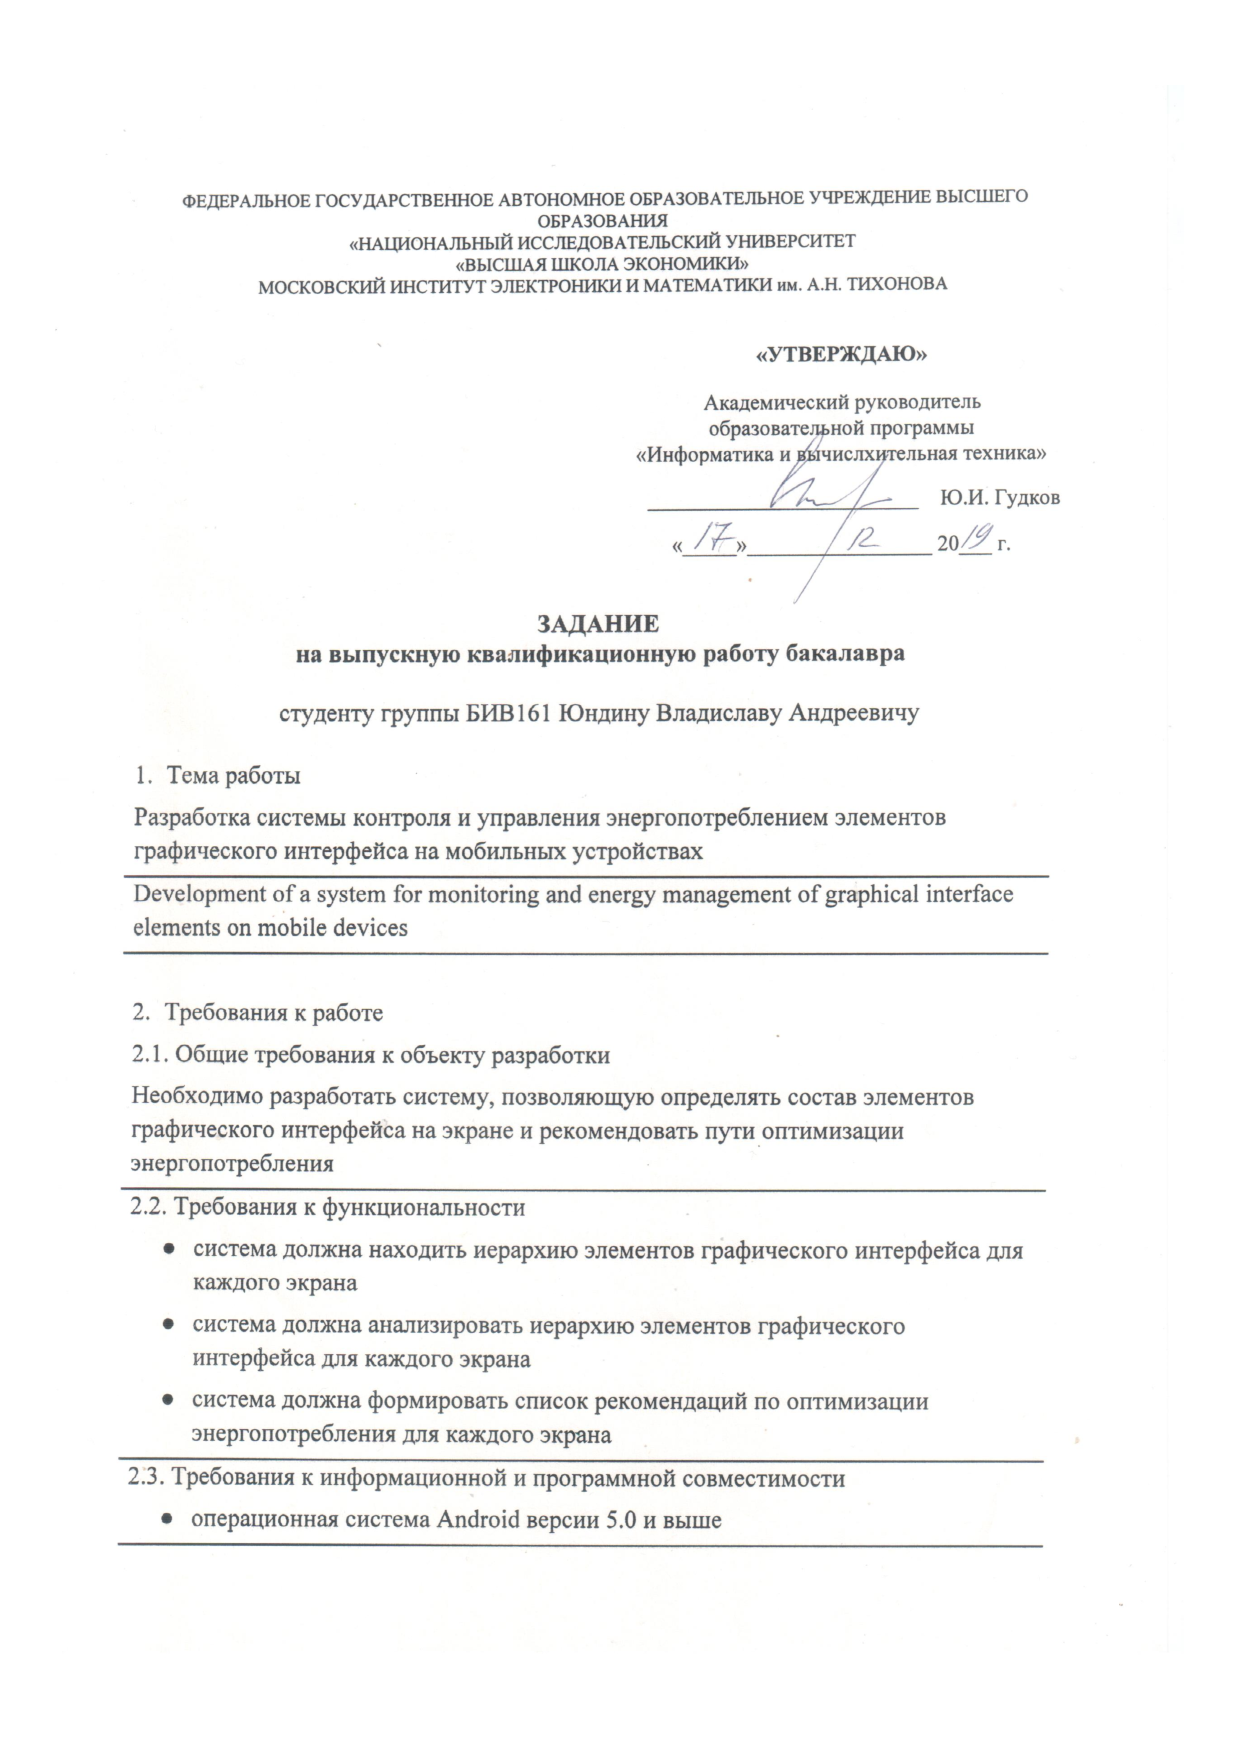
\includepdf[pages=-]{tz.pdf}
	
	\centertitle{Аннотация}
	
	В настоящее время мобильные устройства пользуются большей популярностью, чем когда-либо прежде. Для улучшения опыта взаимодействия с устройствами необходимо более эффективно использовать их ресурсы, особенно важен вопрос разрядки аккумулятора. Целью данной работы является разработка системы контроля и управления энергопотреблением элементов графического интерфейса на мобильных устройствах c операционной системой Android. В работе представлен способ измерения энергопотребления виджетов с помощью анализа отчётов службы batterystats. Процесс измерения управлялся zsh-скриптом через подключение к устройству по USB. Результатом работы стала подключаемая библиотека, способная предложить рекомендации по оптимизации 23 виджетов.
	
	\newpage
	\centertitle{Abstract}
	
	Nowadays mobile devices are more popular than ever before. To improve the experience of interaction with devices it is necessary to use their resources more effectively, especially the battery draining issue is important. The purpose of this paper is to develop a system for monitoring and energy management of graphical interface elements on Android devices. This study presents a method for measuring the power consumption of the widget by analyzing the output of batterystats service. The measurement process was controlled by a script written for zsh while the device is connected via USB. The result is a plug-in library that can offer recommendations for optimizing 23 widgets.
	
	\newpage
	\tableofcontents
	\newpage
	
	%!TEX root = thesis.tex

\centertitletoc{Введение}

Современная жизнь немыслима без смартфонов и разных мобильных приложений, которые могут неэффективно потреблять ресурсы устройства. Значительные проблемы в оптимизации пользовательского опыта возникают в вопросах разряда батареи. Энергоэффективность приложений --- одна из важнейших проблем, с которой сталкиваются как разработчики, так и пользователи~\parencite{man2016experience, wasserman2010software}. Низкая энергоэффективность приложения ускоряет разрядку смартфона и может даже стать основанием для удаления приложения~\parencite{ickin2017users}. Данная проблема имеет популярность среди исследователей, и является предметом большого количества работ. Предложено множество способов снижения энергопотребления, но мне хотелось бы проверить эффективность метода, который основан на замене менее эффективных виджетов на экране более эффективными.

\subparagraph{Цель и задачи}
Конечной целью выпускной квалификационной работы является разработка системы контроля и управления энергопотреблением элементов графического интерфейса на устройствах под управлением операционной системы Android. Для её достижения необходимо решить следующие задачи:
\begin{itemize}
	\item Проанализировать существующие исследования по оптимизации энергопотребления;
	\item Определить инструменты для измерения энергопотребления Android-смартфонов;
	\item Измерить энергопотребление различных элементов пользовательского интерфейса;
	\item Создать библиотеку для мониторинга и управления энергопотреблением графических элементов пользовательского интерфейса
\end{itemize}

\subparagraph{Практическая значимость}
Решение данной проблемы в первую очередь представляет интерес для тех, кто занимается разработкой приложений для Android. Любой инженер, которому важно количество потребляемой приложением энергии, сможет встроить библиотеку в приложение для выявления наиболее затратных элементов интерфейса. Также, полученная библиотека составит список рекомендаций по снижению нагрузки на аккумулятор устройства. Благодаря созданной библиотеке, будет увеличено время автономной работы устройств пользователей.

\subparagraph{Программные средства}
Для разработки системы будет использован язык программирования Kotlin, фреймворк автоматического тестирования пользовательского интерфейса Kaspresso, а также инструмент анализа информации энергопотребления Battery Historian.
	
	\newpage
	\section{Актуальность работы}
	
	Смартфон --- неотъемлемая часть жизни современного человека. Человек может использовать телефон до 200 раз каждый день~\parencite{falaki2010diversity}. Тем не менее, смартфоны всё ещё не достигли потолка своего развития и многие аспекты нуждаются в улучшении. Одним из таких является энергопотребление устройства.
	
	Проблема заключается в том, что с развитием вычислителей и экранов, которые потребляют всё больше энергии, аккумуляторы должны развиваться с сопоставимой скоростью, чтобы покрыть растущие затраты и оставить время работы устройства от батареи хотя бы на том же уровне. Но развитие аккумуляторов устройств происходит не так быстро~\parencite{pentikousis2010search}, что заставляет задуматься о более эффективном расходовании уже имеющейся энергии.
	
	\begin{figure}[htb]
		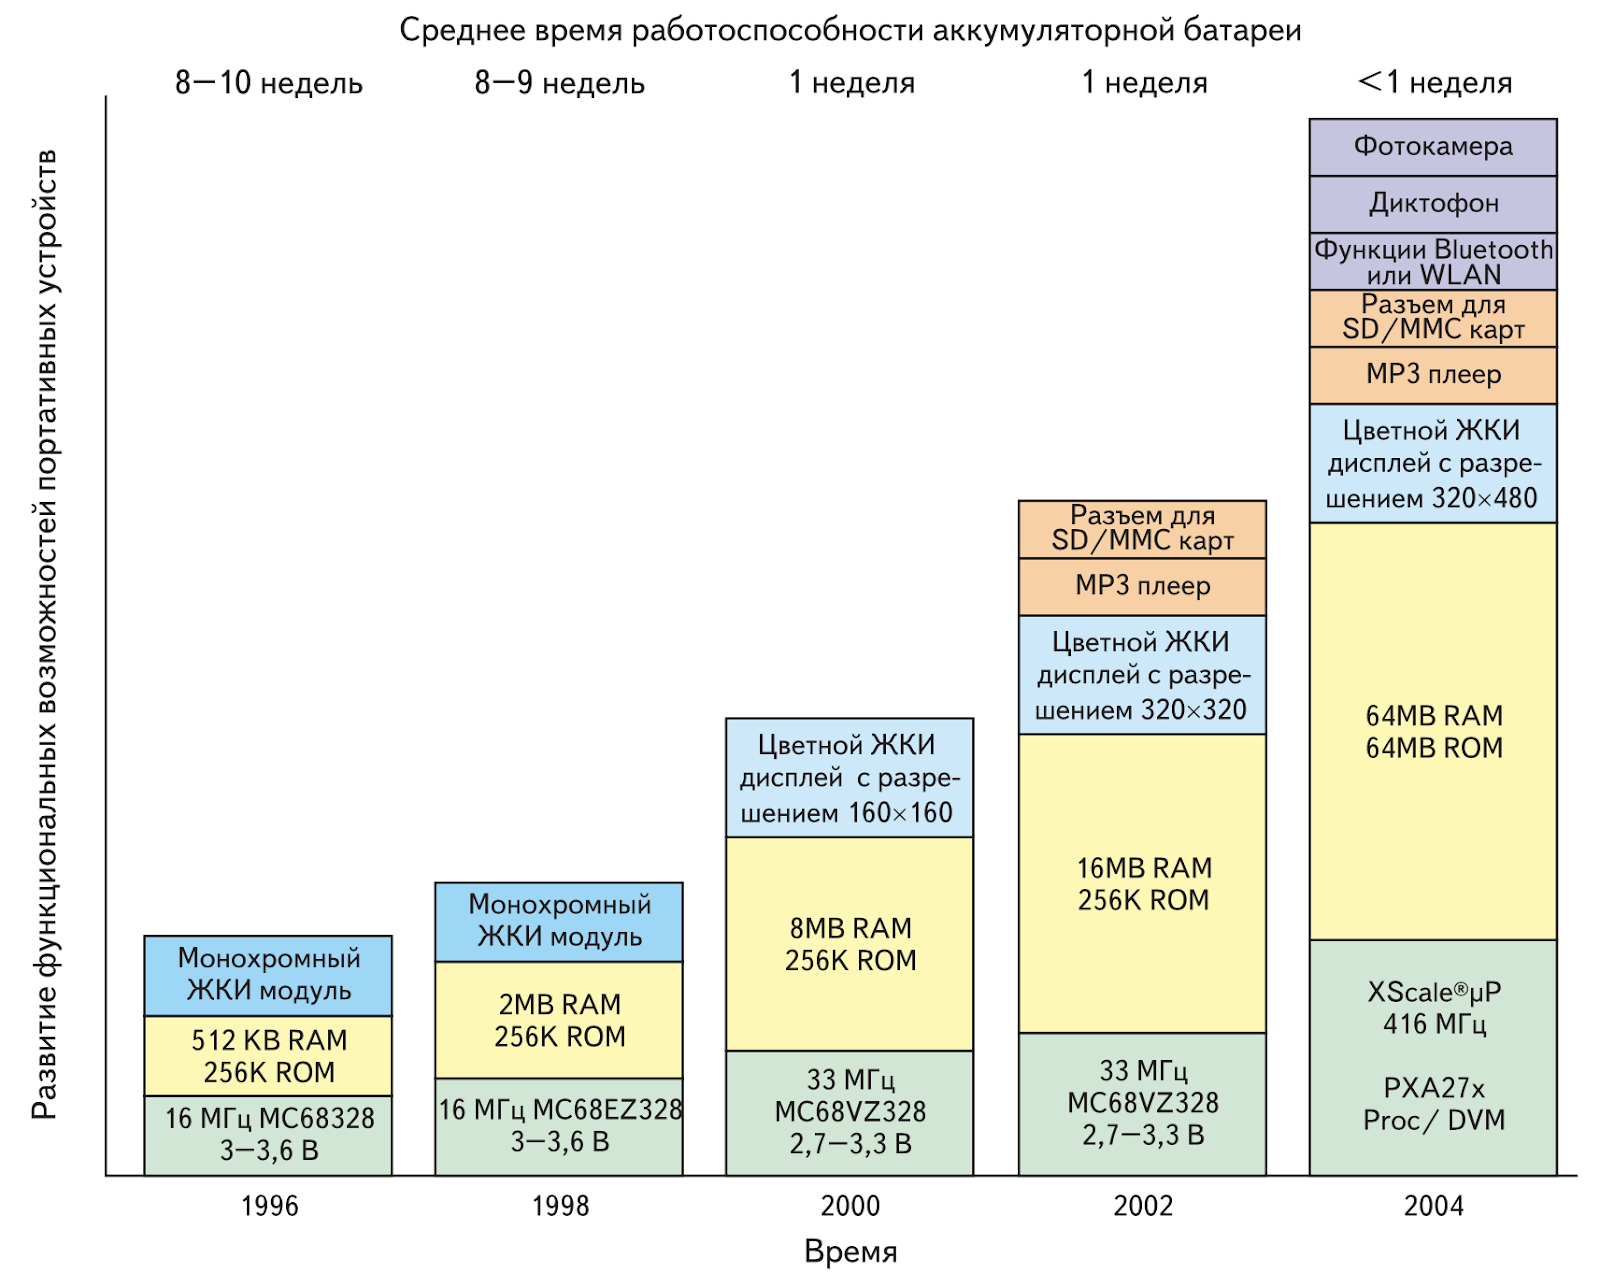
\includegraphics[width=\textwidth]{portable_time}
		\caption{Среднее время работоспособности аккумуляторной батарей}
		\label{fig:portable_time}
	\end{figure}
	
	Раньше мобильные телефоны могли работать более недели от одного заряда аккумулятора, но с их развитием такая возможность была потеряна. Как видно на диаграмме~\ris{\ref{fig:portable_time}}, процесс увеличения числа возможностей портативных устройств сопряжён с уменьшением времени работы прибора. Если в 1996 году портативное устройство было способно работать 8-10 недель до разрядки аккумулятора, то уже в 2004 году наличие камеры, диктофона, Bluetooth, цветного дисплея и другой функциональности сократили время работы до недели и меньше~\parencite{василенко2005методы}.
	
	Существует большое количество факторов, которые влияют на потребление энергии. Это взаимодействие с сетью, множество сенсоров и датчиков, камера, экран и другие. В академических работах показана возможность оптимизировать потребление многих факторов, например, взаимодействие с интернетом~\parencite{tuysuz2019real} или более оптимальное использование оперативной памяти может продлить срок работы устройства от аккумулятора~\parencite{li2014investigation}. Но также исследования показывают, что в большинстве сценариев использования смартфона энергозатраты на экран составляют больше половины всех энергозатрат~\parencite{bai2013android}. Становится очевидным, что именно потребление экрана нуждается в оптимизации в первую очередь.
	
	Имеют место множество подходов к уменьшению потребления экрана, которые основываются на самых разных идеях. Некоторые считают, что изменение цветовой схемы интерфейса на AMOLED экранах поможет снизить затраты~\parencite{wan2015detecting}, другие понижают кадровую частоту и частоту обновления экрана~\parencite{lee2018improving, huang2014intelligent}. 
	
	Новизна моего исследования базируется на предположении, что взаимозаменяемые виджеты со схожей функциональностью потребляют разное количество энергии, что позволяет заменить более затратные виджеты на аналогичные и уменьшить энергопотребление.
	
	Практическое применение моей работы заключается в помощи разработчикам Android-приложений в выборе наиболее эффективных элементов графического интерфейса и улучшение общего качества приложения. Ожидается, что этого удастся достигнуть путём непрерывного сканирования иерархии виджетов с целью поиска тех, которые могут быть заменены на более оптимальные, и сообщения об этом разработчику мобильного приложения.
	
	\newpage
	\section{Обзор литературы}
	
	В этой главе я рассмотрю работы, затрагивающие проблему энергопотребления мобильных устройств и предлагающие пути её решения. Это необходимо для понимания проделанной  исследователями работы, а также изучения методик и инструментов, используемых для проведения измерений.
	
	\subsection{Проблемы пользователей и разработчиков мобильных приложений}
	
	Я считаю необходимым иметь представление о реальных проблемах мобильных приложений как с точки зрения пользователей, так и с позиции разработчиков приложений. Это поможет правильно расставить приоритеты исследования и разработать наиболее удобное и полезное решение по контролю энергопотребления.
	
	Одна из проблем, освещённая в статье Мана, Гао и др., связана с пользовательским восприятием приложений~\parencite{man2016experience}. Авторами был создан новый фреймворк под названием CrossMiner для автоматического анализа проблем приложений из отзывов пользователей с помощью метода, основанного на ключевых словах. Основываясь на пяти миллионах отзывов пользователей, платформа автоматически фиксирует распределение семи проблем приложения, а именно: “батарея”, “сбой”, “память”, “сеть”, “конфиденциальность”, “спам” и “пользовательский интерфейс”. По итогу было выявлено, что проблемы, связанные со “сбоем” и “сетью”, больше беспокоят пользователей, чем другие проблемы на трех рассматриваемых платформах (Google Play, App Store и Windows Store).
	
	\begin{figure}[htb]
		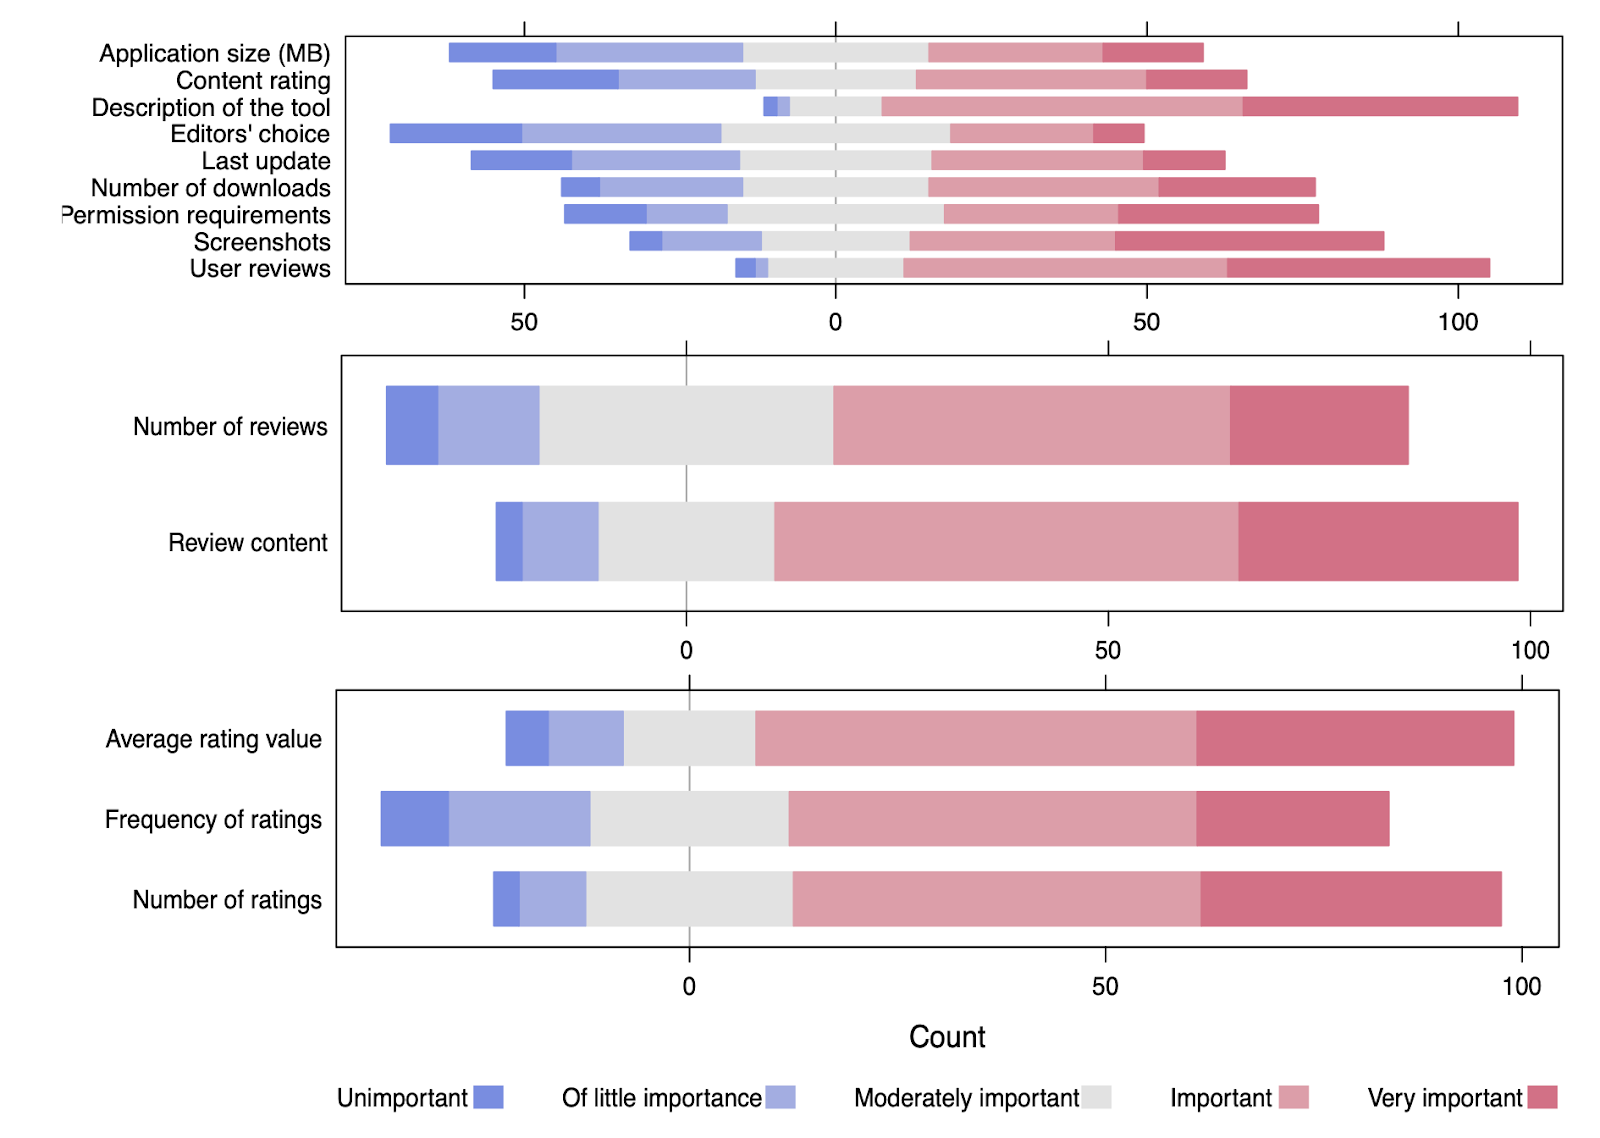
\includegraphics[width=\textwidth]{install_reasons}
		\caption{Причины установки приложений пользователями}
		\label{fig:install_reasons}
	\end{figure}
	
	В другой работе задача состояла в том, чтобы определить причины, по которым пользователи выбирают и устанавливают мобильные приложения из магазинов приложений~\parencite{ickin2017users}. А также причины, по которым пользователи их удаляют. Было проведено анкетирование с участием 121 респондента из 26 различных стран. Как видно на диаграмме \ris{\ref{fig:install_reasons}}, самыми частыми причинами установки приложения являются его описание, оценки пользователей и скриншоты приложения. Согласно другим данным \ris{\ref{fig:delete_reasons}} в топе причин удаления --- бесполезность, сбои, высокое использование оперативной памяти.
	
	\begin{figure}[htb]
		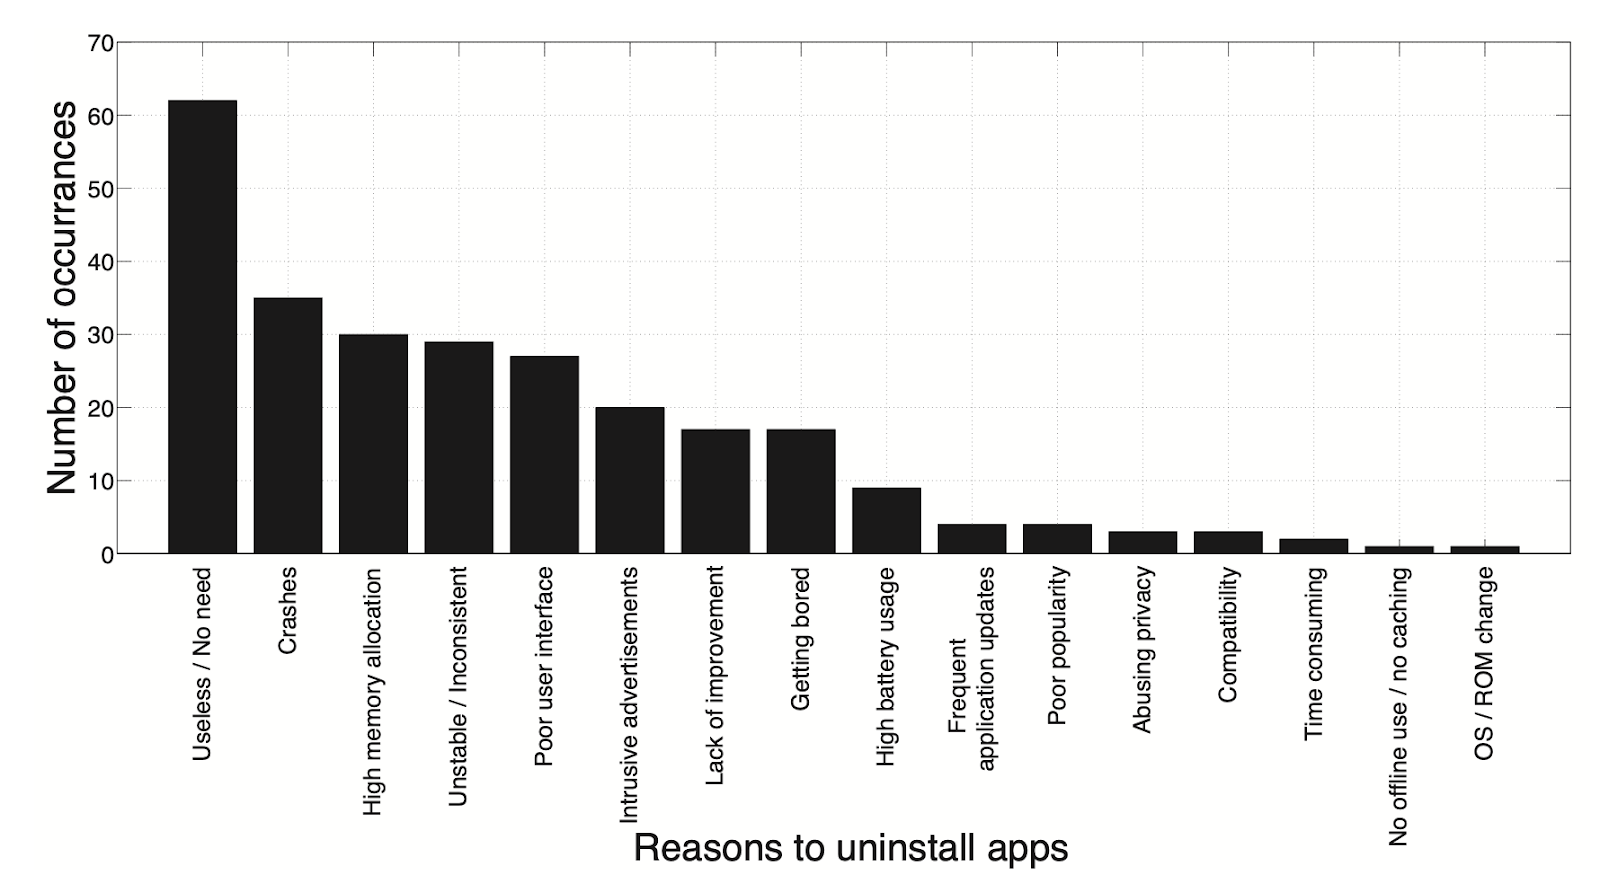
\includegraphics[width=\textwidth]{delete_reasons}
		\caption{Причины удаления приложений пользователями}
		\label{fig:delete_reasons}
	\end{figure}
	
	С точки зрения инженеров~\parencite{wasserman2010software} наиболее остро стоят следующий вопросы: 
	\begin{itemize}
		\item Улучшение пользовательского опыта; 
		\item Нефункциональные требования (производительность, энергоэффективность, надёжность, качество, безопасность);
		\item Процессы, инструменты и архитектура; 
		\item Переносимость на другие платформы. 
	\end{itemize}

	Эти пункты являются лишь подмножеством возможных тем исследований в области разработки программного обеспечения для мобильных приложений, но служат для обозначения широты исследовательских потребностей и возможностей в этой формирующейся области.
	
	\subsection{Измерение энергопотребления устройств}

	Как мы выяснили ранее, понимание энергопотребления компонентов смартфона является одной из ключевых областей интереса для конечных пользователей, а также разработчиков приложений и системного программного обеспечения. Существующая литература предлагает множество решений для эффективного измерения энергопотребления, что помогает определить влияние различных подходов к оптимизации.
	
	В зарубежных исследованиях нередко предлагаются собственные инструменты измерения. Так, в департаменте компьютерных наук университета Ёнсе в Южной Корее, был разработан AppScope --- приложение для автоматического измерения энергопотребления приложений Android с помощью мониторинга активности ядра~\parencite{yoon2012appscope}. Оно отслеживает системные вызовы, а также анализирует данные механизма IPC операционной системы.
	
	В статье Сео, Малека и Медвидовика представлена структура для оценки энергопотребления программных систем на основе Java~\parencite{seo2007energy}. Её инфраструктура использует компонентную перспективу, что делает ее подходящей для большого класса современных распределенных, встроенных и распространяющихся приложений. В большом количестве сценариев распределенных приложений платформа показала очень хорошую точность в целом, давая результаты, которые были в пределах 5\% от фактического потребления энергии, затраченного при работе приложения.
	
	Проектная группа из университета Джорджа Мейсона и Национального института стандартов и технологий США представила систему, которая эффективно учитывает энергопотребление всех основных аппаратных подсистем телефона: процессора, дисплея, графики, GPS, аудио, микрофона и Wi-Fi~\parencite{murmuria2012mobile}. Для этого они использовали доли времени для каждой подсистемы, сообщаемые модулем управления питанием операционной системы. Предложенное решение позволяет работать в режиме реального времени без значительного влияния на энергопотребление подконтрольного устройства, что может помочь разработчикам и исследователям принимать более оптимальные решения для повышения энергоэффективности.

	\subsection{Оптимизации на уровне исходного кода}

	Одним из инновационных подходов к снижению потребления энергии устройством является оптимизация затрат процессорного времени, которое требуется для выполнения вычислительных задач. В данной главе будут рассмотрены пути оптимизации исходного кода программы с целью сокращения времени нагруженной работы процессора и скорейшего его перехода в энергосберегающий режим.
	
	Одно из исследований показало, что JavaScript экономит больше энергии и работает медленнее, чем другие подходы, и что гибридизация приложений может быть решением для оптимизации приложений как с точки зрения производительности, так и энергопотребления~\parencite{oliveira2017study}. Среди двух вариантов гибридизации использование NDK является наиболее безопасным вариантом для повышения производительности, но использование веб-подхода может дать ощутимый результат при небольшом количестве кросс-языковых вызовов.
	
	Ещё одно исследование относительно Java сфокусировано вокруг одного из механизмов для снижения требований к памяти, а именно сжатия~\parencite{гуанджиу2004экономия}. В статье рассматривается влияние сжатия на объём использованных системных ресурсов виртуальной машиной Java (JVM). Также обращается внимание на алгоритмы, применимые для этих целей. Опыты показали, что экономия энергии составляет в среднем 21\%. В тех приложениях, где декомпрессия играет большую роль, результаты заметно хуже.
	
	\subsection{Общие  методы оптимизации потребления ресурсов для портативных устройств}
	
	Многие проблемы энергопотребления приходилось решать ранее для оптимизации различных портативных устройств. Разработанные методы можно применить и для улучшения энергоэффективности смартфонов. 
	
	В статье Маурицио предлагается значительно пересмотреть подход к производству устройств с учётом интересов конечного пользователя~\parencite{маурицио2008переоценка}. А именно: изменить подбор архитектуры и уделять внимание экономии энергии всех стадиях разработки продукта. При выборе архитектуры автор предлагает учитывать критерий энергопотребления, например, энергозатратные архитектуры, использующие ТПЛ и дифференциальные сигнальные методы со скоростью передачи данных более 10 Гбит/с, необходимо сопоставлять с менее энергоёмкими методиками, например, КМОП или использование несимметричных архитектур. В дополнение к данному подходу делается акцент на необходимости дальнейшей оптимизации уже существующих архитектур, дополняя их новыми характеристиками.
	
	Анализ энергопотребления и средней задержки для режима энергосбережения с несколькими циклами ожидания показывает, что можно оптимизировать параметры режимов ожидания с учётом ограничения средней начальной задержки~\parencite{пустовалов2013анализ}. Предложенная автором методика базируется на математической модели для входного потока, которая применима и для сложных систем с большим числом состояний. Однако методика может быть использована лишь для систем, функционирование которых может быть разбито на циклы регенерации.
	
	Также можно рассмотреть более частные случаи. Например, способы по оптимизации потребления энергии устройствами, функционирование которых управляется микроконтроллером. Они нашли себе применение в том числе и в смартфонах. Обзор охватывает программные, архитектурные и схемотехнические способы снижения потребления~\parencite{кафтанников2013оптимизация}:
	\begin{itemize}
		\item Программные способы направлены на снижение вычислительной нагрузки микропроцессора. Приведены такие способы, как использование специфичной математики, так как операции с дробными числами занимают продолжительное время. Также учёт разрядности процессора может сыграть существенную роль в снижении энергопотребления. Ещё один способ предполагает переписывание наиболее ресурсозатратных участков кода на язык ассемблера, но это лишит возможности переноса получившихся решений на другую платформу;
		\item Архитектурные способы применимы разработчиками микроконтроллера и к ним относится реализация различных режимов энергосбережения, что позволяет отключать неиспользуемую периферию, а также снижать тактовую частоту процессора. Также отключение неиспользуемых узлов кристалла позволит в разы снизить потребление энергии;
		\item Схемотехнические методы оптимизации применимы к самой аккумуляторной батарее. Предлагается использование литий-ионных или литий-полимерных источников питания для обеспечения прямого питания схемы от батареи. Также предлагается различное напряжение питания для вычислительного ядра и периферии, но это приводит к снижении тактовой частоты микросхем.
	\end{itemize}
	
	\subsection{Энергопотребление в операционной системе Android}

	Следующая предметная область, которая стоит отдельного упоминания в контексте данной выпускной квалификационной работы, --- энергопотребление в операционной системе Android, так как именно для оптимизации работы этой операционной системы будут использованы результаты работы.
	
	В статье  Ли и Халфонда была проведена эмпирическая оценка общепринятых методов энергосбережения и повышения производительности~\parencite{li2014investigation}. Она позволила определить, в какой степени эти методы смогли сэкономить энергию по сравнению с неоптимизированными аналогами кода. В частности, было обнаружено, что объединение сетевых пакетов до определённого размера и использование определённых методов кодирования для считывания информации о длине массива, доступа к полям классов и выполнения вызовов приводят к снижению энергопотребления. Однако другие методы, такие как ограничение использования памяти, оказали минимальное влияние на количество затраченной энергии. Эти результаты позволят разработчикам избежать использования неэффективных подходов.
	
	Работа Ли, Хао и др. по сбору информации о поведении приложений в контексте энергопотребления выявила, что в среднем приложения тратят 60\% своей энергии в неактивных состояниях. При этом самым энергоёмким составляющим является взаимодействие устройства с сетью~\parencite{li2014empirical}. Также они проанализировали три распространённых метода, используемых в исследованиях, связанных с измерением энергопотребления: использование времени работы для расчёта приближенного значения; использование измерения на уровне миллисекунд; и пренебрежение затратами энергией в состоянии покоя. Существенный недостаток этих методов заключается в большой погрешности измерения, что может исказить результаты исследований.
	
	\subsection{Оптимизация энергопотребления экранов мобильных устройств}
	
	Целевым компонентом результата данной работы --- системы для оптимизации энергопотребления элементов графического интерфейса --- является экран мобильного устройства. В связи с чем стоит рассмотреть ранее изученные подходы к энергооптимизации данного компонента.
	
	Исследования показывают, что потребление может быть уменьшено за счет снижения частоты кадров~\parencite{lee2018improving}, оптимизации сети~\parencite{tuysuz2019real}, использования памяти~\parencite{li2014investigation}, использования тёмного фона жидкокристаллических экранах~\parencite{утин2018адаптивное} и так далее. Эмпирическое исследование показывает, что смартфон потребляет большое количество энергии при отображении интерфейса для пользователя~\parencite{li2014empirical}. 
	
	Ван и Джин~\parencite{wan2015detecting} описали методику обнаружения энергоёмких интерфейсов и их преобразования для экономии энергии. Их результаты оказали значительное влияние на оценку энергопотребления экрана и, кроме того, их идея была разработана в исследовании Линареса-Васкеса и др.~\parencite{linares2018multi}. Суть данного подхода основана на оптимизации цветовой палитры при сохранении допустимого уровня контрастности. Частота обновления дисплея также была изучена научным сообществом. Хуан и др.~\parencite{huang2014intelligent} и Ким и Юнг~\parencite{kim2014content} предполагают, что частота обновления является ключевым фактором, за счёт снижения которого достигается экономия энергии.
	
	Ключевой особенностью исследования Вана и Джина~\parencite{wan2015detecting} является инструмент, который может анализировать содержимое скриншота. Это модель потребляемой дисплеем мощности, которая предсказывает количество энергии, потребляемой каждым пикселем экрана, принимая во внимание тип экрана и цвет определённого пикселя. Позже оригинальный скриншот трансформируется, чтобы достичь более энергоэффективного пользовательского интерфейса. Преобразованное изображение аналогично анализируется перед сравнением результатов с исходными данными. Результаты работы учёных показывают, что предполагаемая экономия энергии достигает 50\% от первоначального значения. Это указывает на то, что их идеи служат хорошей основой для дальнейшего изучения. В данной работе оценка погрешности модели была измерена только на 4 различных устройствах, которые могут не отражать полноту всей картины.
	
	В работе Линарес-Васкес и др.~\parencite{linares2018multi} основой подхода является многоцелевое рассмотрение контента. Это позволяет разработчикам достичь компромисса между тремя выделенными целями: снижение энергопотребления на OLED-дисплеях, увеличение контраста между соседними элементами пользовательского интерфейса и сохранение согласованности в использовании цветов по сравнению с оригинальным дизайном. Для достижения такого поведения необходимо найти состояние оптимальности по Парето, в котором улучшение одной из целевых функций не может быть достигнуто без ухудшения других целей. С помощью указанных методов учёным удалось в некоторых случаях снизить энергопотребление на 79\%. Этот результат представлен с множеством графически выраженных данных, которые иллюстрируют весь процесс. Вопрос, который остаётся нераскрытым --- это сопоставимость опыта пользователя до и после оптимизации питания.
	
	Хуан и др.~\parencite{huang2014intelligent}, в свою очередь, демонстрируют взаимосвязь между энергопотреблением и частотой обновления дисплея. В настоящее время частота обновления ЖК-экранов постоянна, что приводит к тому, что экрану приходится рисовать те же кадры без особой на то необходимости. Учёные представили механизм, сокращающий избыточные обновления кадров и доступ к памяти на основании информации о кадровых буферов. Тем не менее, из исследования невозможно сделать вывод об устройствах с типом экрана, отличным от LCD.
	
	В дополнение к вышеупомянутым исследованиям Ким и Юнг~\parencite{kim2014content} придерживались идеи интеллектуальной частоты обновления дисплея. Ключевой особенностью статьи является показатель скорости контента и его отношение к частоте обновления экрана. Предлагаемая метрика скорости контента начинается с определения частоты обновления контента для каждого приложения и затем управления частотой обновления, чтобы оптимизировать энергопотребление без ущерба для пользовательского восприятия. Измерение частоты обновления контента основано на частоте кадров и сравнении кадровых буферов разных кадров для вычитания избыточной частоты кадров. Кроме того, была применена технология ускорения касанием: частота обновления резко возрастает, когда происходит событие касания. Это исследование все ещё имеет некоторые ограничения: только одна модель устройства была протестирована, а типы дисплеев, для которых исследование является действительным, не описаны.
	
	\subsection{Выводы}
	
	Проведённый обзор литературы показал, что на текущий момент проблема энергопотребления активно разрабатывается исследовательским сообществом. Авторы показали необходимость оптимизации ПО, разработки инновационных программных и аппаратных решений, а также учёта пользовательского восприятия. Тем не менее, остаётся открытым вопрос дальнейшей проработки решений, которые помогут повысить энергоэффективность дисплея как самого энергозатратного компонента смартфона.
	
	\newpage
	\section{Инструменты измерения энергопотребления}
	
	Измерение энергопотребления приложения в конкретный момент или небольшой промежуток времени --- одна из самых важных и сложных задач, которую необходимо решить в ходе выполнения выпускной квалификационной работы.
	
	Необходимость в проведении таких измерений связана с необходимостью формирования базы данных элементов пользовательского интерфейса и советов для их оптимизации. В ходе работы системы контроля и управления энергопотребления сформированная база элементов пользовательского интерфейса будет использоваться для сравнения данных по энергопотреблению текущих элементов с подобными по выполняемой функциональности и поиска наиболее энергоэффективных альтернатив.
	
	\subsection{Способы измерения}
	
	Для получения энергопотребления конкретного приложения могут быть использованы следующие подходы:
	\begin{itemize}
		\item анализ напряжения на аккумуляторе, получаемого через компонент приложения BroadcastReceiver;
		\item получение данных по энергопотреблению с помощью инструмента Android Profiler;
		\item анализ данных по конкретному приложению, собираемых операционной системой, с помощью инструмента Battery Historian;
		\item анализ напряжения на аккумуляторе, собираемого операционной системой, с помощью Battery Historian;
		\item измерение энергопотребления всего устройства с помощью стороннего оборудования.
	\end{itemize}

	Анализ напряжения, получаемого через BroadcastReceiver страдает от несовершенности API. Разные устройства могут иметь различное поведение относительно частоты обновления данных, но в среднем новое значение рассылается при уменьшении заряда аккумулятора на один процент. То есть данный подход позволяет получить лишь около 100 значений за время полного разряда устройства, чего недостаточно для анализа.
	
	Android Profiler и Battery Historian позволяют фильтровать потребление по отдельному приложению, что несомненно является преимуществом. Но Android Profiler не учитывает потребляемую экраном энергию и показывает лишь потребление по четырёхзначной шкале (None, Low, Meduim, High) следующих потребителей: процессор, сеть, геолокация. Этого также не хватит для полноценного анализа.
	
	Battery Historian отображает более точную информацию о потреблении конкретным приложением. Доступна информация по проценту израсходованной батареи, а также процессорное время, использованное приложением. Но доступны только суммарные данные за всё время с последней полной зарядки устройства. То есть нельзя сказать, сколько потребляло приложение в конкретный момент времени. Так как тесты проводятся в рамках одного приложения, использовать Battery Historian без модификаций не получится. 
	
	Данные по напряжению в Battery Historian доступны по временным промежуткам, но они довольно хаотичны \ris{\ref{fig:historian_voltage}} и без информации о силе тока, ничего извлечь из них не получится.
	
	\begin{figure}[htb]
		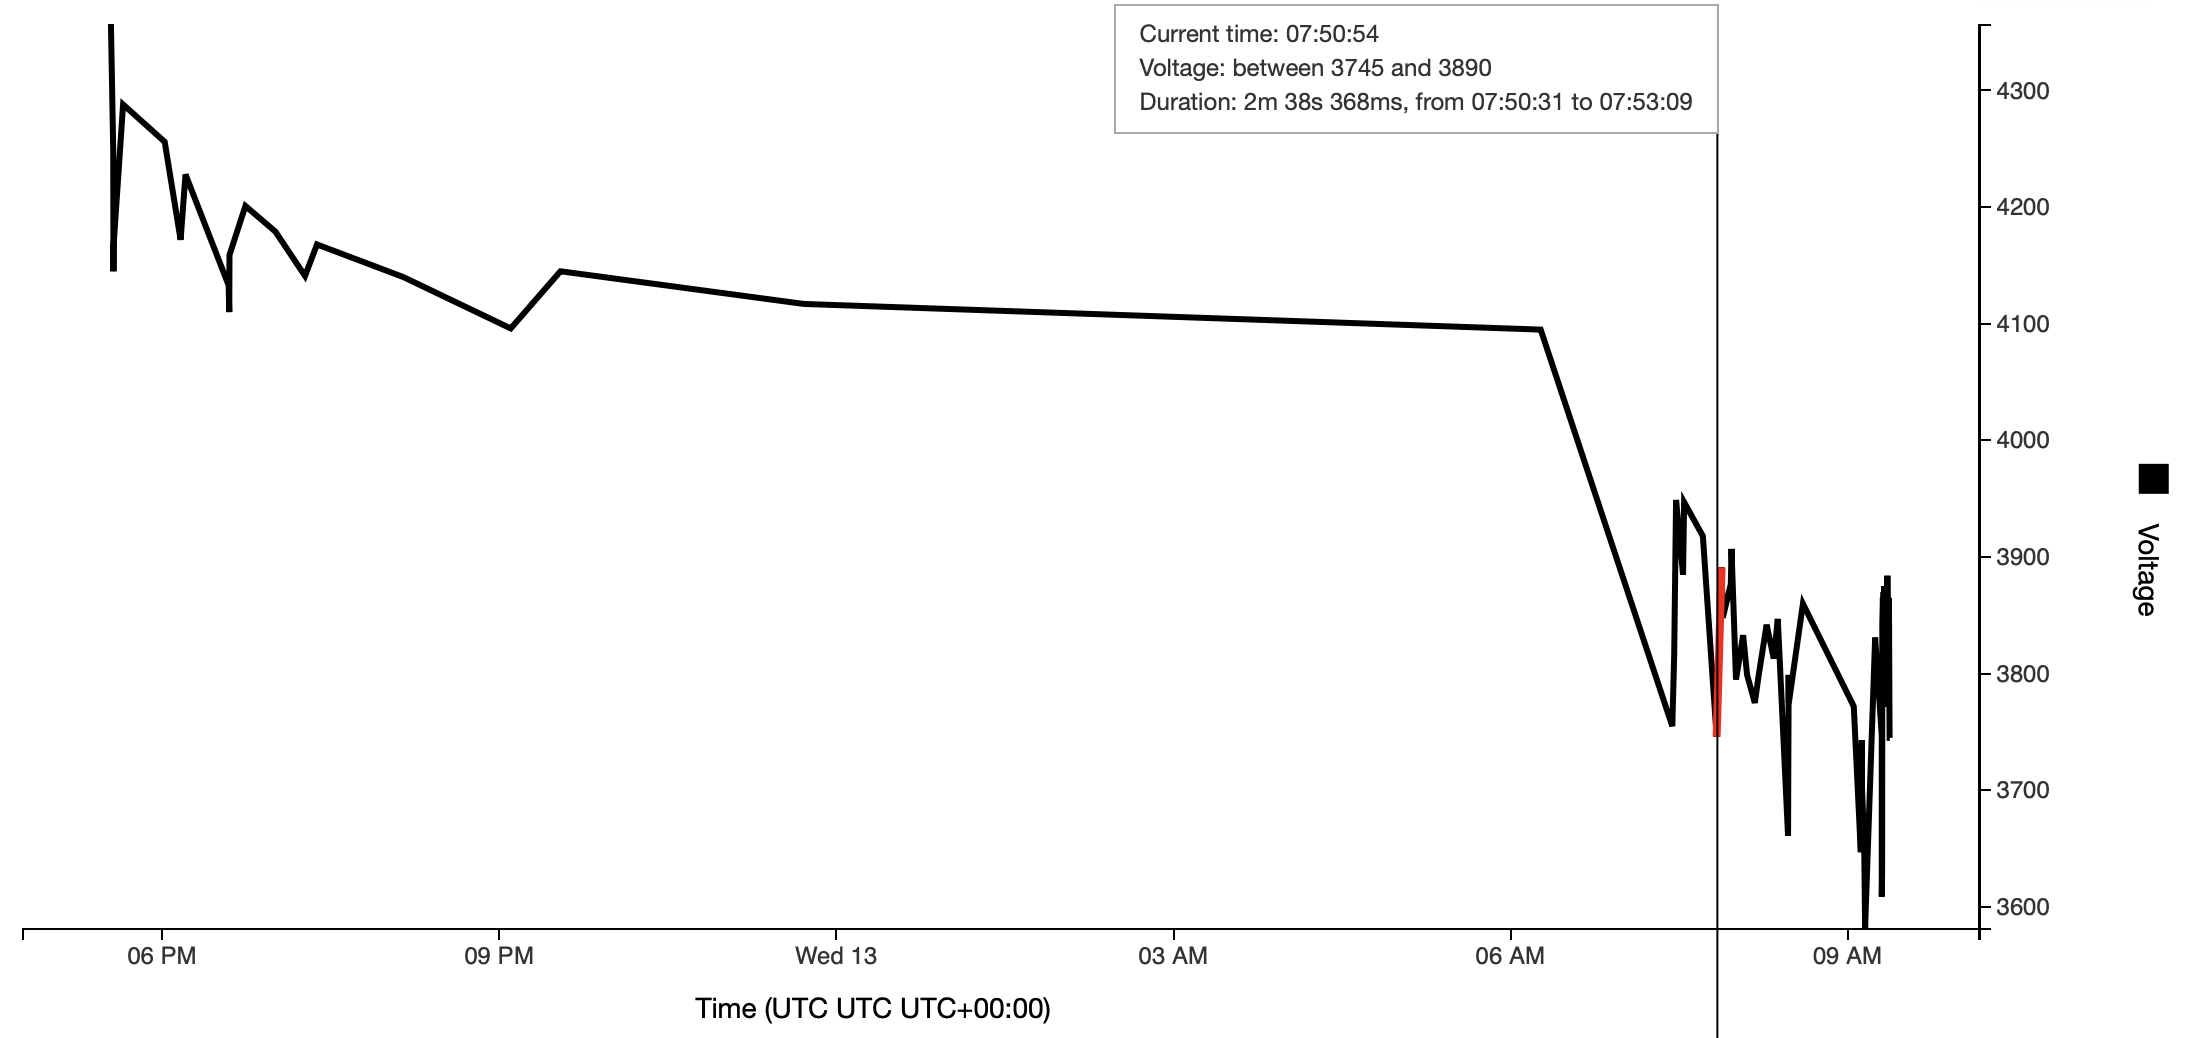
\includegraphics[width=\textwidth]{historian_voltage}
		\caption{Напряжение на аккумуляторе устройства}
		\label{fig:historian_voltage}
	\end{figure}

	Из-за недостатков остальных подходов, изначальный выбор был сделан в пользу измерения энергопотребления с помощью стороннего оборудования.
	
	\subsection{Обоснование выбранного инструмента}
	
	Самым надёжным способом в настоящий момент остаётся измерение потребления всего устройства с помощью стороннего оборудования. Данный подход используется практически всеми современными исследованиями, требующими измерения энергопотребления приложения. Устройство для измерения подключается к тестируемому устройству вместо аккумуляторной батареи и записывает показатели потребляемой устройством мощности с некоторым интервалом. Устройства для измерения варьируются от платы Arduino с небольшой программой до оборудования, специально созданного для таких целей. Самым популярным решением является использование Monsoon Power Monitor, именно его я собирался использовать при проведении собственных измерений.
	
	К сожалению, доставка устройства или его аналогов не представляется возможным, в связи с чем, при измерениях придётся данные операционной системы.
	
	Данные ОС выводит в текстовом виде, после чего они могут быть загружены для анализа в Battery Historian. Но так как файлы текстовые, для сокращения времени их анализа, они могут быть проанализированы собственными алгоритмами. К сожалению, найти документации к содержимому файлов не удалось, поэтому формат их содержимого пришлось анализировать самостоятельно.
	
	\subsection{Анализ системных отчётов}
	
	В Battery Historian загружается zip-архив, получаемый через Android Debug Bridge командой \textbf{adb bugreport}. Его следует проанализировать в первую очередь.
	
	\subsubsection{Анализ архива отчёта}
	
	При распаковке архива мы получаем директорию c файлами, описанными в документации~\parencite{BugreportFormat}:
	\begin{itemize}
		\item bugreport-OnePlus3-PKQ1.181203.001-2020-05-13-12-21-11.txt --- самый большой по занимаемому дисковому пространству файл, содержащий всю основную информацию;
		\item FS --- директория с некоторыми данными из файловой системы устройства;
		\item dumpstate\_log.txt --- файл, содержащий информацию о том, как прошёл сбор данных;
		\item lshal-debug --- директория с информацией о слоях аппаратных абстракций операционной системы;
		\item main\_entry.txt --- файл, содержащий имя файла с основными данными, в данном случае, первого в списке файла;
		\item proto --- информация от вспомогательных служб в proto-формате;
		\item version.txt --- файл с версией формата отчёта, данном случае используется версия 2.0.
	\end{itemize}

	После изучения директории становится понятно, что единственный файл, представляющий интерес --- первый в списке.  При открытии файла мы видим шапку с информацией о модели устройства, версии ядра операционной системы и так далее \ris{\ref{fig:report_header}}. После этого упоминается вызов инструмента \textbf{dumpsys} и представлены разделённые на блоки отчёты различных служб.
	
	\begin{figure}[!htb]
		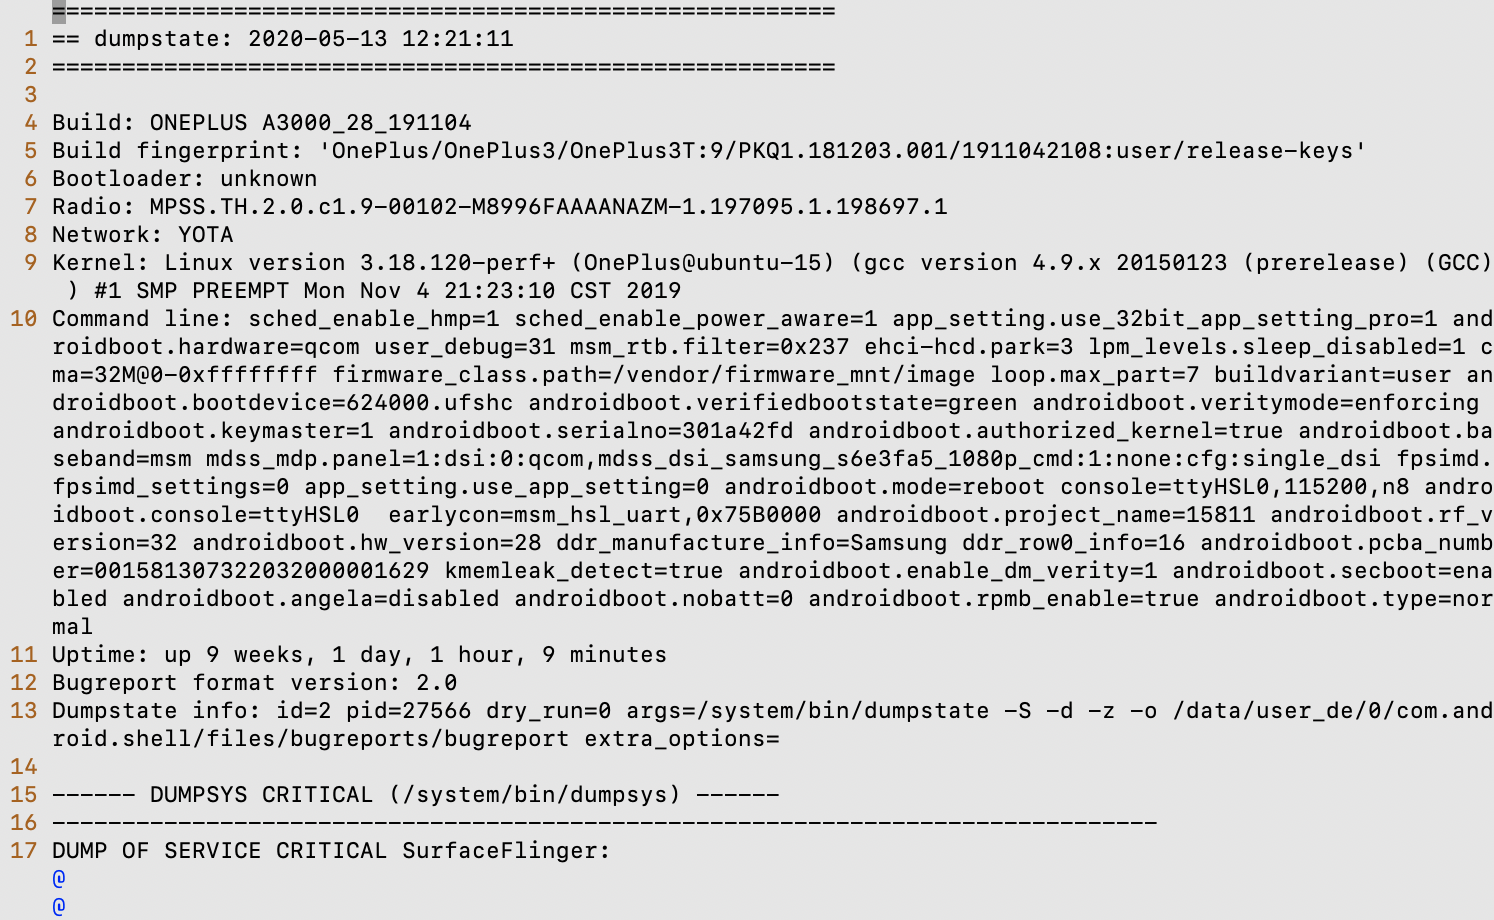
\includegraphics[width=\textwidth]{report_header}
		\caption{Шапка отчёта устройства}
		\label{fig:report_header}
	\end{figure}

	\subsubsection{Инструмент dumpsys} \label{subsub:dumpsys}
	
	Из найденной документации к \textbf{dumpsys}~\parencite{Dumpsys} становится понятно, что отчёты служб можно получать по отдельности, что удобно, так как файл отчёта, полученный из архива, содержит более 500 тысяч строк и понадобится далеко не вся информация, которую он содержит. В документации можно найти команду \textbf{adb shell dumpsys batterystats}, которая возвращает статистику по расходу заряда батареи устройства. Возвращаемый файл достаточно объёмный, наибольший интерес представляет раздел \textbf{Statistics since last charge}, так как он содержит информацию по конкретным приложениям.
	
	В подразделе \textbf{Estimated power use (mAh)} отображаются затраты, разделённые на Uid~\ris{\ref{fig:estimated_use}}. Uid --- это пользовательский идентификатор в Unix-подобных операционных системах, он уникален для каждого приложения и по нему можно отслеживать энергопотребление и затраченное процессорное время.
	
	\begin{figure}[!htb]
		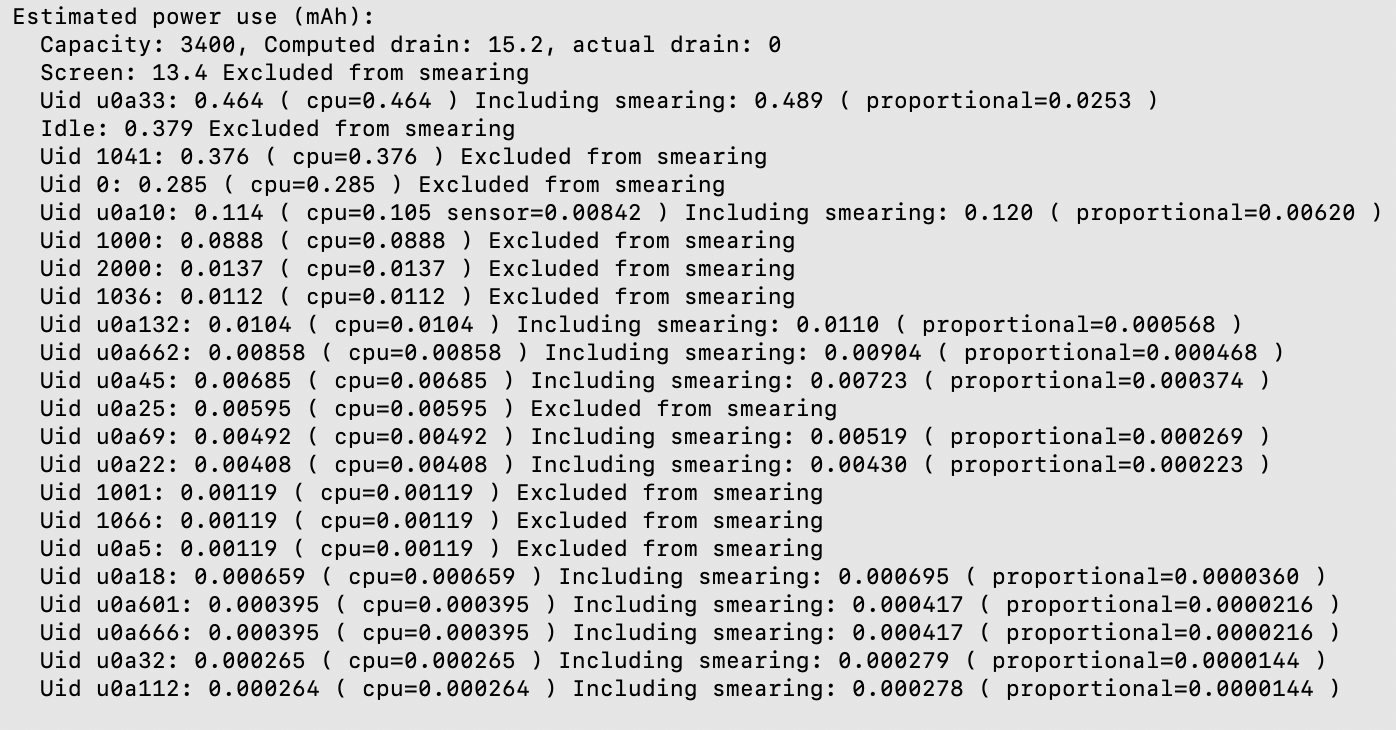
\includegraphics[width=\textwidth]{estimated_use}
		\caption{Подраздел с затратами на каждый Uid}
		\label{fig:estimated_use}
	\end{figure}
	
	Также в разделе есть подраздел с общей статистикой для каждого Uid в системе, там не указана израсходованная энергия, но есть информация о процессорном времени, потраченным на это приложение~\ris{\ref{fig:uid_subsection}}.

	\begin{figure}[!htb]
		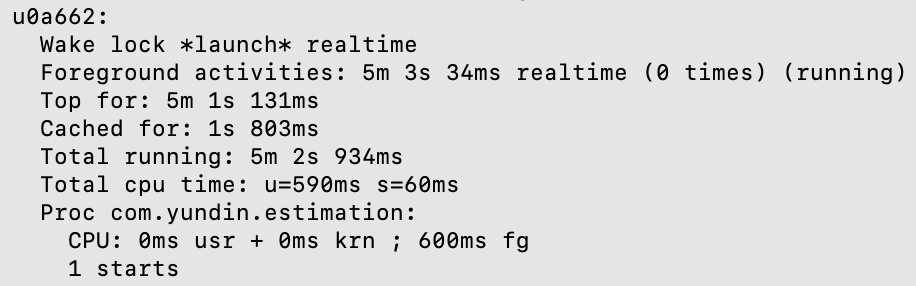
\includegraphics[width=\textwidth]{uid_subsection}
		\caption{Подраздел со статистикой по Uid u0a662}
		\label{fig:uid_subsection}
	\end{figure}

	Также была использована служба \textbf{cpuinfo}, предоставляющая дополнительную информацию о затраченном процессорном времени. Обычно сервис предоставляет незначительную информацию, но в отчётах устройства, используемого для тестирования (OnePlus A3000), имелись дополнительные данные, разделённые по времени и Uid, что предоставляет возможности для дополнительного анализа~\ris{\ref{fig:cpuinfo}}.
	
	\begin{figure}[H]
		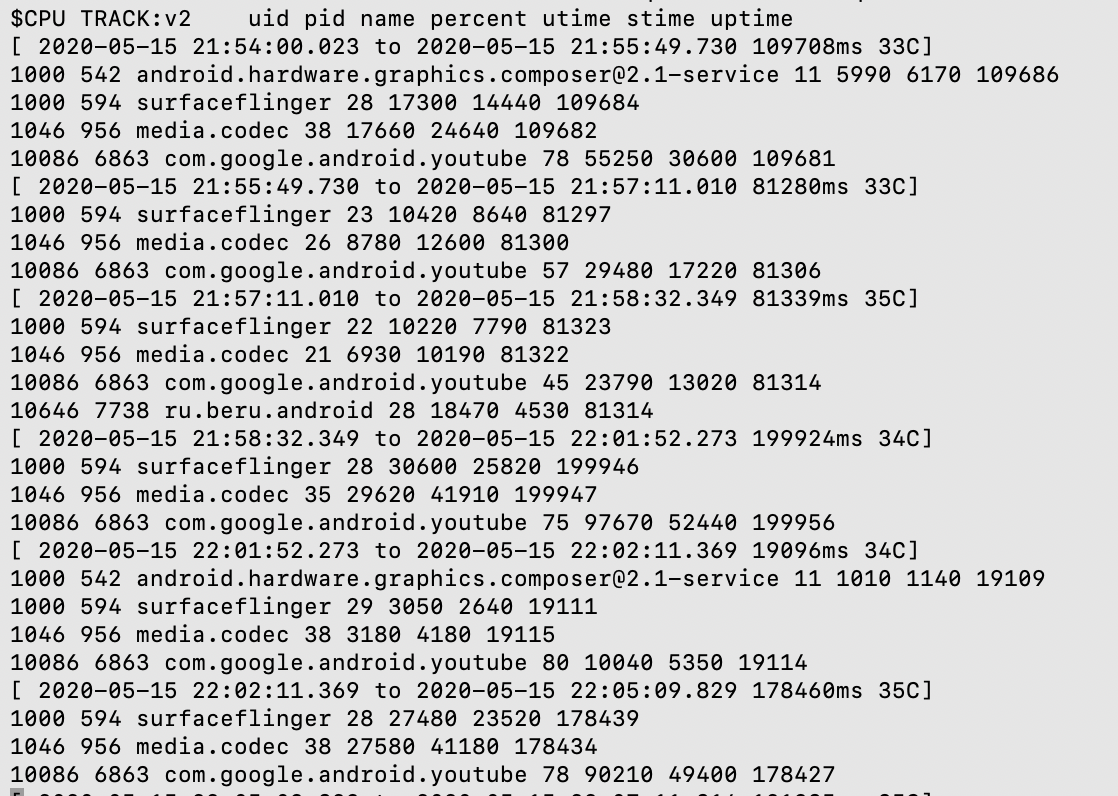
\includegraphics[width=\textwidth]{cpuinfo}
		\caption{Дополнительная информация сервиса cpuinfo на устройстве OnePlus A3000}
		\label{fig:cpuinfo}
	\end{figure}

	Получаемые с помощью служб \textbf{batterystats} и \textbf{cpuinfo} данные уже не содержат нерелевантную информацию от других служб операционной системы, но всё ещё имеют объём 3-5 тысяч строк. Понадобится инструмент фильтрации нужной информации.

	\subsection{Фильтрация данных}
	
	На первом этапе фильтрации нужно оставить только информацию, которая относится к тестируемому приложению. 
	
	\subsubsection{Служба batterystats}
	
	Для службы \textbf{batterystats} это строка с нужным Uid из подраздела \textbf{Estimated power use (mAh)}, а также подраздел с общей статистикой по Uid. Для фильтрации этой информации на языке Python был написан скрипт \textbf{filter\_bat.py}. Скрипт принимает в качестве аргументов командной строки имена файлов, которые ему требуется отфильтровать. Отфильтрованные версии файлов помещаются в директорию \textbf{batt\_results\_filtered/}, которую создаёт скрипт.
	
	\subsubsection{Служба cpuinfo}
	
	Из службы \textbf{cpuinfo} понадобятся такие строки, которые отражают данные для промежутка времени, в которое производилось тестирование, и содержат информацию по Uid тестируемого приложения. Также понадобятся сами строки с датами, так как временные промежутке в файле не равные. Для фильтрации данных на языке Python был написан скрипт \textbf{filter\_cpu.py}. Он так же принимает в качестве аргументов командной строки имена файлов, которые ему требуется отфильтровать, а результат помещает в созданную директорию \textbf{cpu\_results\_filtered/}.

	\newpage
	\section{Процесс сбора данных}
	
	Сложность проведения измерений энергопотребления приложения заключается в наличии большого количество факторов, влияющих на показатели энергопотребления, которые не связаны непосредственно с работой приложения. Такими факторами могут быть другие приложения, выполняющие работу в фоновом режиме, задачи операционной системы, а также особенности конкретного устройства.
	
	\subsection{Оптимизация сбора данных} \label{sub:optimization}
	
	 Избавиться от влияния всех факторов не представляется возможным, однако для уменьшения их влияния можно предпринять следующие меры:
	\begin{itemize}
		\item проводить тестирование на устройстве без сторонних приложений;
		\item проводить тестирование на устройстве с операционной системой без сервисов Google Play Services, которые выполняют фоновые задачи операционной системы;
		\item проводить тестирование всех элементов интерфейса на одном и том же устройстве;
		\item проводить тестирование при активированном на устройстве режиме полёта;
		\item проводить тестирование с максимальной яркостью экрана.
	\end{itemize}

	К сожалению, доступа к устройству без сторонних приложений и с операционной системой без сервисов Google Play Services, не имеется. Тестирование будет проводится на устройстве OnePlus A3000 с операционной системой Android 9 и версией ядра 3.18.120-perf+. На устройстве будет активирован режим полёта и установлена максимальная яркость экрана. Также будут закрыты все сторонние приложения.

	Несмотря на то, что данные меры снижают погрешность при измерениях, они не исключают её полностью. Поэтому будет необходимо провести несколько измерений и дополнительно обработать результаты, чтобы получить усреднённые значения.
	
	\subsection{Проблемы при сборе данных}
	
	Используемый метод получения данных от операционной системы не лишён недостатков. Стоит их рассмотреть.
	
	\subsubsection{Сброс статистики}
	
	Как уже упоминалось, служба Battery Historian предоставляет только суммарные данные за время с последней полной зарядки устройства, что мешает получать данные по конкретному виджету. Такое поведение обусловлено тем, что именно в таком формате предоставляет данные служба \textbf{batteryststs}, анализ которой будет производится и в этой работе.
	
	Для решения данной проблемы была использована команда \textbf{adb shell dumpsys batterystats -{}-reset}, которая помогает вручную сбросить все имеющиеся данные и начать запись статистики сначала. 
	
	В случае сброса данных перед измерением определённого виджета и сбора статистики после измерения, полученные данные будут отражать статистику по конкретному виджету, что и требуется.
	
	\subsubsection{Связь с компьютером} \label{subsub:connection}
	
	Для сбора результатов измерения виджета и сброса статистики перед измерением следующего может понадобится подключение устройства к компьютеру, который будет вызывать эти команды через Android Debug Bridge.
	
	Подключение может быть осуществлено через USB-кабель, либо через локальную сеть, когда устройства подключены к одной точке доступа Wi-Fi.
	
	В случае общей точки доступа, устройство имеет доступ к интернету, что не позволит ему находится в режиме полёта и может сильно исказить результаты при обращении других приложений к сети. Данный способ подключения далее не рассматривается.
	
	В случае подключения по кабелю устройство находится в состоянии зарядки. Однако когда устройство заряжается, сбор статистики службой \textbf{batteryststs} приостанавливается. Для решения этой проблемы была использована возможность искусственно выключать режим зарядки на устройстве командой \textbf{adb shell dumpsys battery set usb 0}. После команды устройство продолжает заряжаться, но операционная система ведёт себя так, будто устройство не заряжается. Очевидно, что в этом случае результаты также могут быть неточными, поэтому искажения данного способа будут дополнительно рассмотрены в подразделе~\ref{sub:nousb_test}.
	
	\subsection{Автоматизация процесса}
	
	Как стало понятно в подразделе \ref{subsub:dumpsys}, между переключением элементов нужно обращаться к командной оболочке операционной системы устройства, чтобы записывать статистику по протестированному элементу на компьютер и сбрасывать её перед тестированием следующего.
	
	В теории, это может быть сделано двумя способами: обращением к командной оболочке из самого приложения, либо обращением к оболочке через средства Android Debug Bridge с компьютера. При проверке оказалось, что первый вариант невозможен, так как требует особого разрешения операционной системы, которое не выдаётся сторонним приложениям~\parencite{Dump_Permission}. Поэтому сбор и сброс статистики необходимо осуществлять через Android Debug Bridge. 
	
	Механизмов обращения из приложения к компьютеру не предусмотрено. Поэтому сделан вывод о том, что тестом должен управлять скрипт, который исполняется на компьютере, он будет сбрасывать данные, запускать измерения с нужным виджетом и записывать результат.
	
	Был написан zsh-скрипт \textbf{estimation.sh}~\ris{\ref{fig:estimation}}, который в цикле для каждого виджета сбрасывает статистику батареи и запоминает время начала теста. Так как способ запуска измерений пока неизвестен, в коде оставлены пустые строки. После запуска измерений, скрипт ожидает до окончания теста плюс одну секунду, после чего записывает время окончания теста, а также собранную статистику. После выполнения измерений для каждого виджета, записывается статистика процессора.
	
	\begin{figure}[htb]
		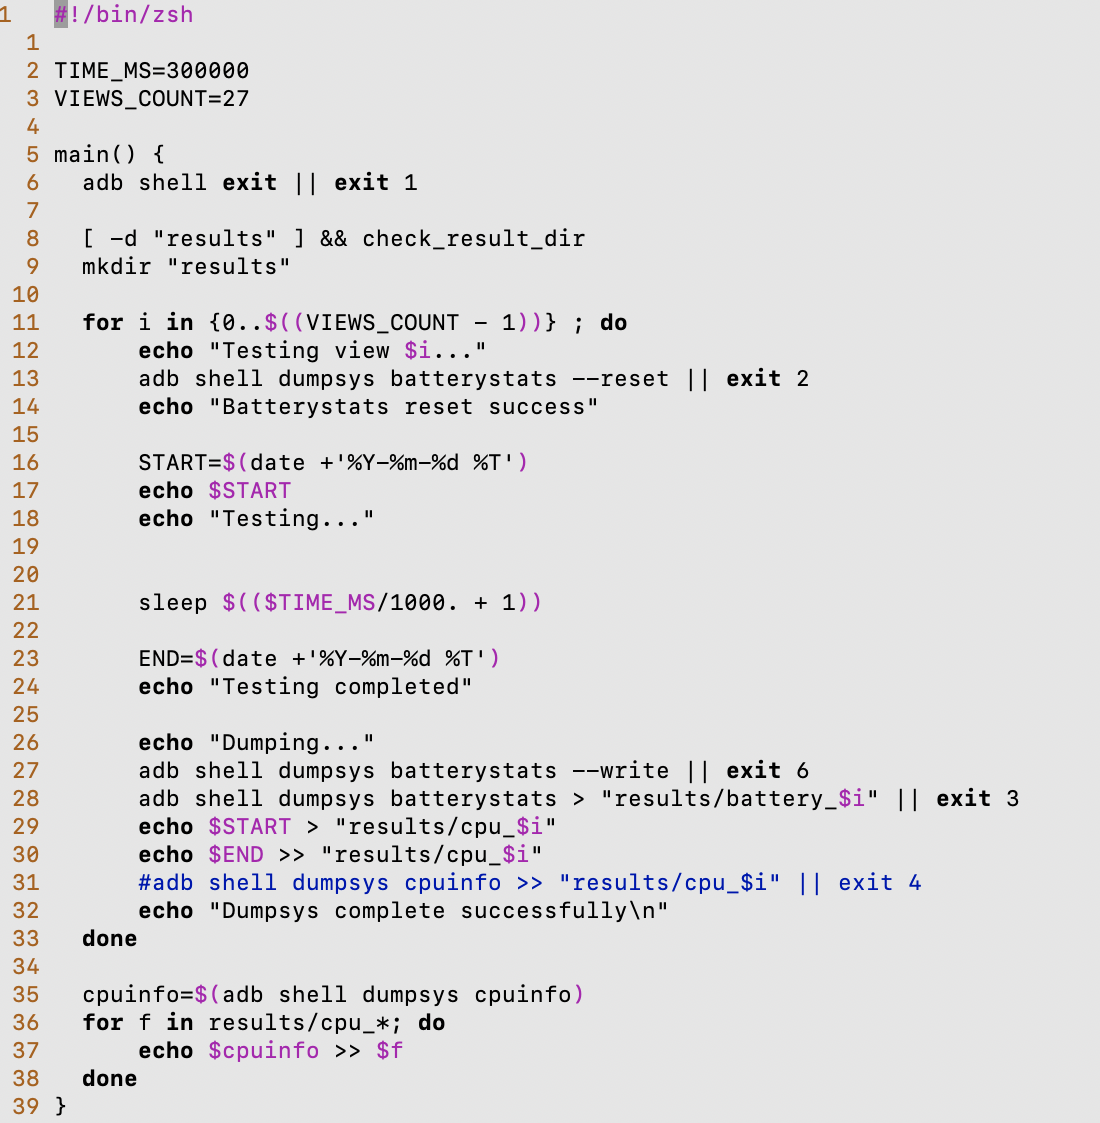
\includegraphics[width=\textwidth]{estimation}
		\caption{Листинг части скрипта для проведения измерений}
		\label{fig:estimation}
	\end{figure}
	
	Запись времени начала и конца необходима, чтобы найти результат тестирования в статистике процессора. Она не сбрасывается вместе со статистикой батареи, поэтому необходимо записать время, в которое проводился тест, в файл со статистикой. Статистика процессора отображается за промежуток в последние несколько суток.
	
	\clearpage
	\section{Составление списка элементов}
	
	До начала всех измерений необходимо конкретизировать круг всех элементов интерфейса, с которыми итоговая система будет корректно работать.
	
	Было решено использовать только те виджеты, которые могут быть отображены без взаимодействия с другими виджетами, следовательно, могут быть измерены отдельно от всего остального. В противном случае, было бы необходимо измерять виджеты во всех возможных условиях, а это бы в разы увеличило время проведения тестов.
	
	Для составления списка элементов был взят список всех сущностей пакета android.widget в Android 10 SDK Platform (\hyperref[appendix]{Приложение}). После этого из списка были исключены следующие сущности:
	\begin{itemize}
		\item deprecated классы, так как они не рекомендуются к использованию разработчиками ОС и в будущих версиях могут быть удалены;
		\item интерфейсы и классы-адаптеры, так как они не являются виджетами;
		\item абстрактные классы, так как невозможно создать объект такого класса;
		\item вспомогательные классы, так как они не являются виджетами;
		\item виджеты, требующие наличие адаптера или презентера для отображения;
		\item наследники представлений, задачей которых является позиционирование других представлений, добавленных к текущему.
	\end{itemize}
	
	После этого остался список самостоятельных элементов, которые можно независимо тестировать:
	\begin{itemize}
		\item AutoCompleteTextView
		\item Button
		\item CalendarView
		\item CheckBox
		 \item CheckedTextView
		 \item Chronometer
		 \item DatePicker
		 \item EditText
		 \item ImageButton
		 \item ImageSwitcher
		 \item ImageView
		 \item MultiAutoCompleteTextView
		 \item NumberPicker
		 \item ProgressBar 
		 \item RadioButton
		 \item RatingBar
		 \item SearchView
		 \item SeekBar
		 \item Space
		 \item Switch
		 \item TextClock
		 \item TextSwitcher
		 \item TextView
		 \item TimePicker
		 \item ToggleButton
		 \item VideoView
		 \item View
		
	\end{itemize}
	
	\clearpage
	\section{Измерение одного виджета}
	
	Ручное проведение измерений потребует огромного количества времени для включения экранов с различными элементами интерфейса, а также данное переключение будет неточным и может исказить результаты. Поэтому необходимо разработать средства, позволяющие автоматизировать процесс отображения нужного виджета.
	
	Чтобы управлять отображением виджетов на экране, был выбран инструментарий для автоматического тестирования графического интерфейса. Он позволяет имитировать реальное взаимодействие пользователя с устройством. В этой работе пользовательские действия не будут имитированы, но это может понадобится для дальнейших исследований.
	
	\subsection{Проектирование автоматических тестов}
	
	Автоматические тесты графического интерфейса помогут отображать виджеты на экране по команде, поданной компьютером. Это избавляет от необходимости ручного управления переключением элементов и искажений, которые накладывает ручное переключение.
	
	Однако в подразделе \ref{subsub:connection} была обозначена необходимость сравнения результатов измерений в условиях подключения к компьютеру по кабелю и отсутствия такого подключения. Это важно, потому что запуск автоматических тестов без подключения к компьютеру невозможен. 
	
	\subsubsection{Процесс запуска Activity}\label{subsub:activity_start}
	
	Появляется необходимость запускать тестирование не только через автоматические тесты, но и с запуском Activity. Запуск Activity может быть произведён как с компьютера, так и без взаимодействия с ним. Также появляется необходимость сравнения результатов измерений при отображении виджета через запуск автотеста и запуск Activity. Результат такого сравнения представлен в подразделе~\ref{sub:test_act}.
	
	Для создания максимально близких условий последующего сравнения, процесс создания объекта виджета и его добавления к Activity должны быть одинаковы при отображении виджета через запуск автотеста и запуск Activity.
	
	Для достижения такого поведения, именно Activity на стадии своей инициализации должна иметь информацию о номере виджета, и устанавливать его на экран. После чего Activity должна ждать столько, сколько нужно для тестирования виджета, и завершаться. 
	
	Передать информацию об индексе нужного виджета, а также о времени тестирования можно единственным способом: через объект Intent, с помощью которого происходит запуск Activity. Intent может быть сформирован как через adb, так и при запуске Activity через автотест, что создаёт одинаковые условия запуска Activity.
	
	При создании класса Activity создаётся массив всех виджетов. В методе onCreate Activity получает необходимые данных из объекта Intent, создаёт объект класса нужного виджета, устанавливает его в качестве своего наполнения, а также создаёт отложенную задачу на своё завершение, которую помещает в очередь сообщений главного потока. Последнее действие нужно потому, что метод onCreate всегда вызывается в том же потоке исполнения, в котором происходит отрисовка пользовательского интерфейса, и если заставить поток ждать, виджет не будет отображён на экране.
	
	Теперь для запуска измерений нужного виджета через автотест, необходимо лишь сконфигурировать Intent запуска Activity, запустить её и не завершать поток исполнения автотеста до завершения тестирования. Если поток автотеста завершится сразу после запуска Activity, то завершится и сама Activity. Так как в данном случае не имитируется взаимодействие пользователя с виджетом, поток не выполняет никакой работы, а просто ожидает.
	
	\subsubsection{Передача данных при запуске теста}
	
	Ещё одна проблема появляется при передаче номера тестируемого виджета автотесту. По умолчанию возможности передавать дополнительные данные из команды запуска теста в код теста нет, но её можно добавить, расширив класс Instrumentation. По умолчанию, в приложении используется класс AndroidJUnitRunner в качестве Instrumentation, поэтому мой класс MyTestRunner будет наследовать и расширять возможности AndroidJUnitRunner~\ris{\ref{fig:mytestrunner}}.
	
	\begin{figure}[tbh]
		\includegraphics[width=\textwidth]{mytestrunner}
		\caption{Листинг класса MyTestRunner}
		\label{fig:mytestrunner}
	\end{figure}
	
	Было решено передавать в приложение 2 параметра: индекс виджета и время его тестирования. Время будет удобнее определять в единственном месте, этим местом будет zsh-скрипт. После этого остаётся в файле \textbf{build.gradle} сменить testInstrumentationRunner на написанный com.yundin.estimation.MyTestRunner.
	
	\subsubsection{Обработка объекта виджета}
	
	Некоторые элементы, например TextView или ImageView, требуют наполнения каким-нибудь содержимым, чтобы отображаться на экране. Некоторые элементы требуют менее тривиальных манипуляций перед отображением. Чтобы унифицировать процесс обработки элемента перед и после добавления на экран, было принято решение создать класс ViewWrapper, который будет содержать класс требуемого представления, а также методы beforeAdd и afterAdd, которые будут вызваны до добавления на экран и после добавления на экран соответственно.
	
	Если элементу требуются дополнительные действия, как в примерах выше, методы могут быть переопределены в наследниках класса ViewWrapper. При отображении виджета производятся следующие действия:
	\begin{enumerate}
		\item Создаётся объект класса представления, содержащегося в объекте ViewWrapper;
		\item Вызывается метод beforeAdd для созданного объекта;
		\item Объект устанавливается в качестве наполнения Activity;
		\item Вызывается метод afterAdd для добавленного объекта.
	\end{enumerate}

	Были написаны наследники класса ViewWrapper, которые будут наполнять виджеты минимальным содержимым \ris{\ref{fig:wrapper}}. В Activity будет формироваться массив, содержащий объект ViewWrapper для каждого тестируемого виджета.
	
	\begin{figure}[tbh]
		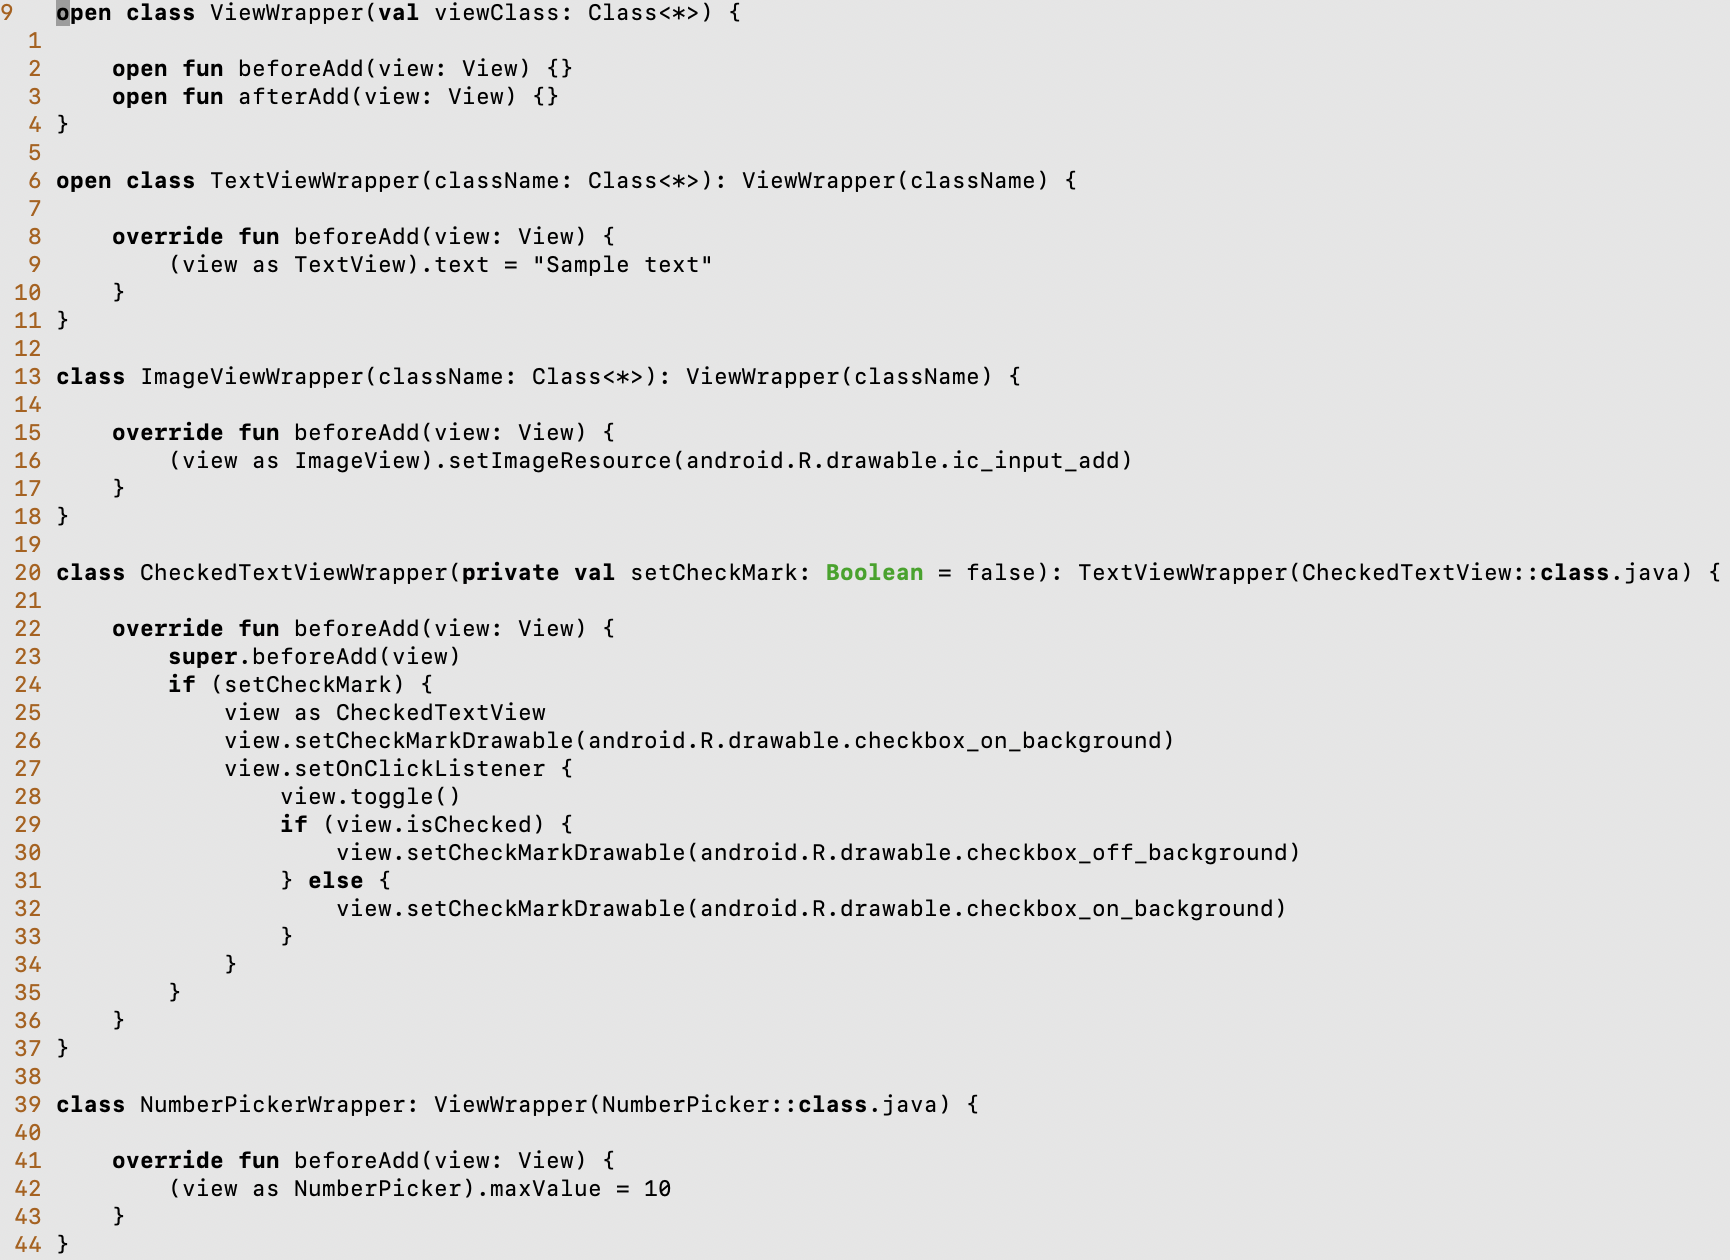
\includegraphics[width=\textwidth]{wrapper}
		\caption{Листинг класса ViewWrapper и части его наследников}
		\label{fig:wrapper}
	\end{figure}
	
	\subsection{Выбор фреймворка автоматического тестирования}
	
	Далее необходимо выбрать конкретный инструмент, позволяющий писать автотесты для Android, рассмотрим варианты:
	\begin{itemize}
		\item appium;
		\item espresso;
		\item kakao;
		\item kaspresso.
	\end{itemize}
	
	Appium не является подходящим, так как он не всегда стабильно работает, а также не поддерживает старые версии Android. 
	
	У Espresso подобные проблемы отсутствуют, но присутствует проблема с избыточностью синтаксиса и нечитаемости итогового кода. 
	
	Kakao и Kaspresso в свою очередь основываются на Espresso, но каждый по-своему исправляет избыточность синтаксиса с помощью возможностей языка Kotlin, но Kaspresso имеет расширенную функциональность, поэтому был выбран данный фреймворк.
	
	\clearpage
	\section{Сравнение результатов измерений в разных условиях}
	
	В подразделах~\ref{subsub:connection} и~\ref{subsub:activity_start} обосновывается необходимость сравнения результатов измерений, проведённых в разных условиях.
	
	\subsection{Влияние подключённого USB-кабеля} \label{sub:nousb_test}
	
	В этом подразделе будут протестированы сценарии измерений при подключённом USB-кабеле с искусственно отключённым режимом зарядки и при питании только от батареи.
	
	Условия тестирования будут максимально похожими, они описаны в подразделе~\ref{sub:optimization}. Единственное отличие, помимо подключения к зарядке, будет в способе запуска Activity. 
	
	В случае подключения к компьютеру запуск будет происходить также, как при реальных измерениях, с помощью команды \textbf{adb shell am start}. В случае отсутствия связи с компьютером, приложение будет запускаться через нажатие на его иконку в списке приложений.
	
	При открытии приложения через нажатие на иконку, будет сформирован Intent без информации о том, какой виджет и на какое время нужно отобразить. Поэтому при отсутствии этих данных в Intent Activity будет использовать значения по умолчанию, они же будут переданы при запуске через adb.
	
	Тестирование будет производится с виджетом, имеющим номер ноль, а именно AutoCompleteTextView. Перед тестом статистика будет сброшена, после теста статистика будет сохранена в файл. Каждый сценарий повторяется трижды, чтобы увидеть искажения от подключения к сети, а также разницу между измерениями, проведёнными по одному сценарию.
	
	\begin{figure}[H]
		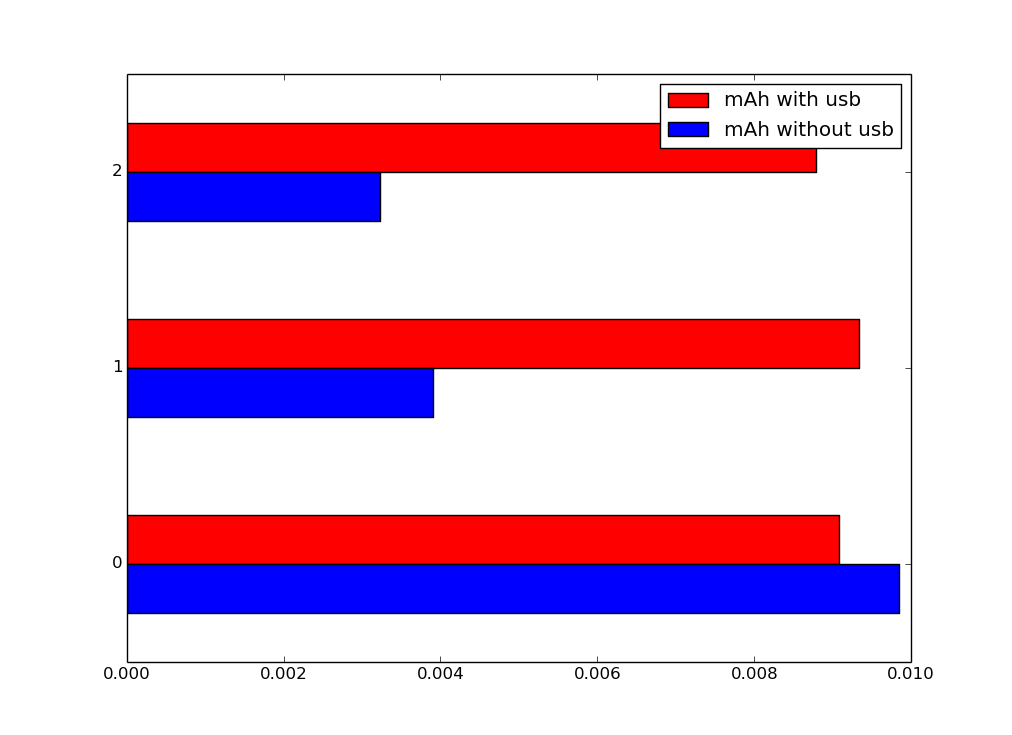
\includegraphics[width=\textwidth]{usb_comparation}
		\caption{Результаты сравнения сценариев измерения. Красные столбцы --- 3 измерения с подключённым кабелем. Синие столбцы --- к устройству ничего не подключено.}
		\label{fig:usb_comparation}
	\end{figure}

	Сравнение показало, что результаты измерения по разным сценариям достаточно сильно отличаются~\ris{\ref{fig:usb_comparation}}, но разница между измерениями без подключения к компьютеру также довольно большая и такому способу доверять сложно. В то же время при подключённом кабеле результаты относительно стабильные.
	
	\subsection{Влияние запуска через автотест} \label{sub:test_act}
	
	Так как в данном случае не будет имитироваться взаимодействие с пользователем, проводить измерения с помощью автотестов необязательно, можно напрямую запускать Activity, передавая нужные параметры. Необходимо сравнить между собой сценарий измерения с использованием автотестов и с запуском Activity напрямую.
	
	Тестирование так же будет производится на виджете AutoCompleteTextView. Автотест будет запущен командой \textbf{adb shell am instrument}. Activity, как и ранее, запускается командой \textbf{adb shell am start}.
	
	Стоит отметить, что с точки зрения Activity эти сценарии совершенно ничем не отличаются. Она запускается одинаковым образом и совершает одинаковые действия.
	
	\begin{figure}[tbh]
		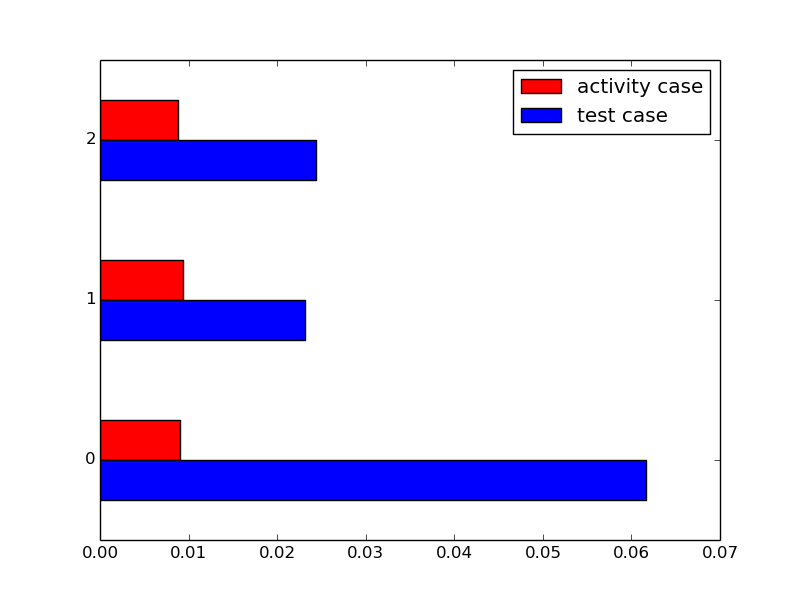
\includegraphics[width=\textwidth]{test_comparation}
		\caption{Результаты сравнения  сценариев измерения. Красные столбцы --- измерения, запущенные через Activity. Синие столбцы --- измерения, запущенные через автотест.}
		\label{fig:test_comparation}
	\end{figure}

	Результаты представлены на рис.~\ref{fig:test_comparation}. Видно, что измерения, запущенные через автотесты, тратят больше энергии, что можно объяснить издержками на дополнительный поток и исполнение дополнительного кода, запускающего процесс тестирования. Также между результатами трёх одинаковых измерений, запущенных через автотесты, есть существенная разница. Причиной этому могут быть индивидуальные особенности используемого устройства или установленной операционной системы.
	
	Сравнение сценариев измерения показало, что стабильней всего себя показывает вызов Activity напрямую при подключённом USB-кабеле. Для реализации данного сценария для всех виджетов скрипт \textbf{estimation.sh} был модифицирован до скрипта \textbf{activity\_estimation.sh}~\ris{\ref{fig:activity_estimation}}.
	
	\begin{figure}[tbh]
		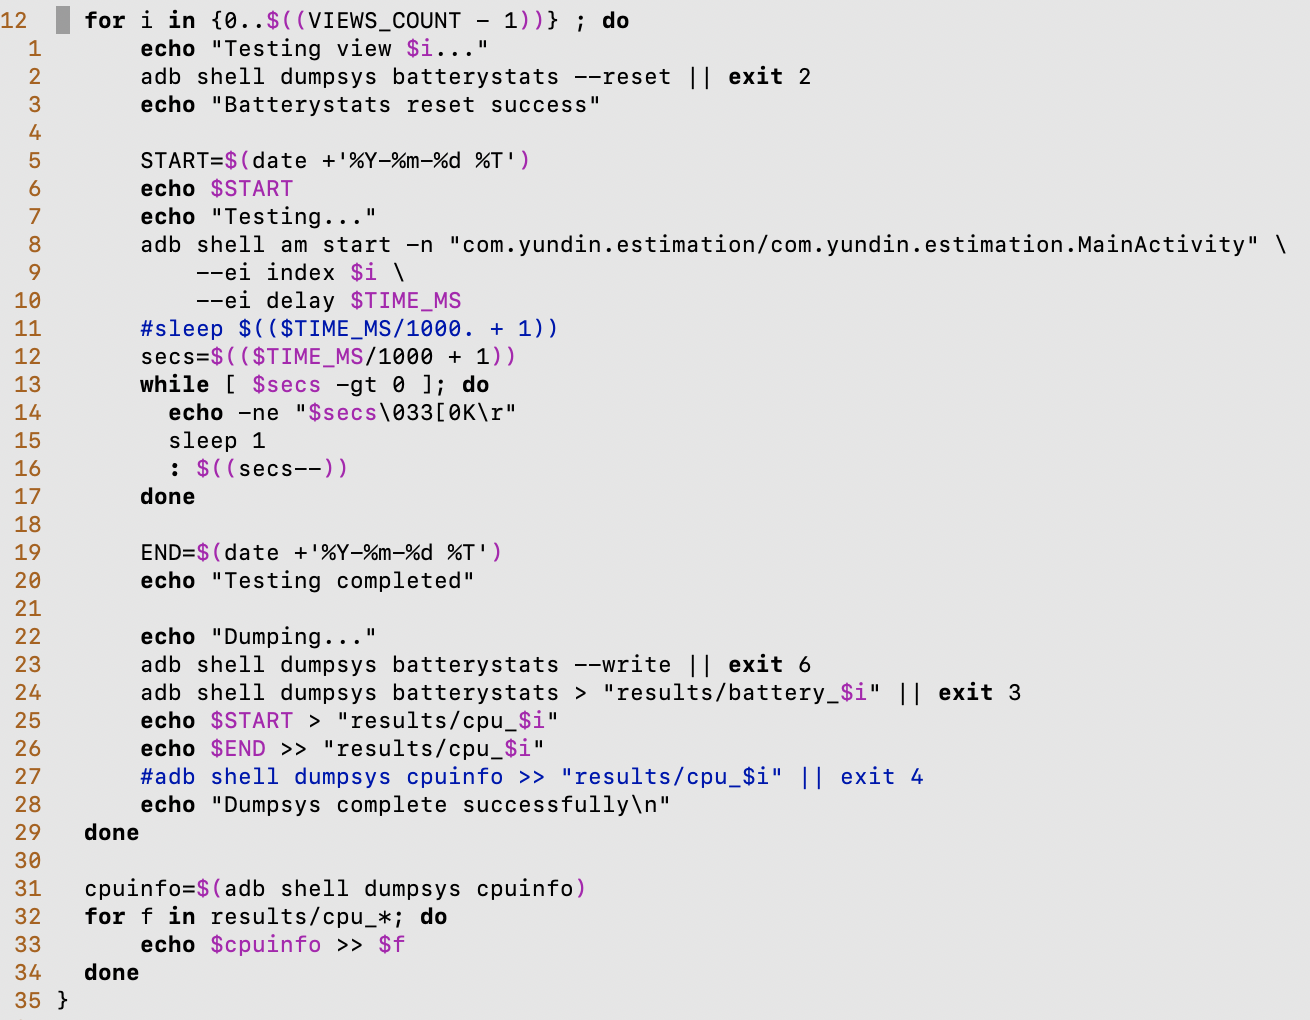
\includegraphics[width=\textwidth]{activity_estimation}
		\caption{Листинг части скрипта activity\_estimation.sh}
		\label{fig:activity_estimation}
	\end{figure}

	\clearpage
	\section{Постобработка результатов измерений}
	
	В ходе сравнения результатов измерений в разных условиях было обнаружено, что тестируемое приложение не отображается в логах службы \textbf{cpuinfo}. Это может быть связано с низкими значениями затрат процессорного времени. Информация этой службы в будущем использована не будет.
	
	После работы скрипта \textbf{filter\_bat.py} файлы содержат только информацию по тестируемому приложению, но она понадобится не в полном объёме. Для сравнения достаточно получить затраченное процессорное время, а также количество mAh.
	
	Скрипт \textbf{concat\_filtered.sh} исключает из ранее отфильтрованных данных все подробности, кроме описанных выше. Также происходит сбор данных для всех виджетов в один файл для удобства дальнейшей обработки.
	
	Скрипт \textbf{sum\_cpu.py} помогает просуммировать процессорное время, потраченное на исполнение системного и пользовательского кода во время работы приложения. Изначально данные представлены в формате, понятном человеку (например, \textbf{u=240ms s=50ms}), но компьютер сравнивать такие строки не сможет. Скрипт переводит данную строку в количество миллисекунд и записывает следующей строкой.

	Скрипт \textbf{median.py} подставляет реальные имена виджетов вместо их номеров и считает медианное значение всех измерений. Используется именно медианное значение, так как из тестов сценариев понятно, что могут наблюдаться выбросы, сильно искажающие среднее значение. 
	
	И наконец, скрипт \textbf{chart.py} сортирует результаты разных виджетов по затраченному процессорному времени и отображает в виде диаграммы.
	
	\clearpage
	\section{Результаты измерений}
	
	Время измерения каждого виджета было установлено на 5 минут. Увеличение времени измерения одного виджета привело бы к существенному увеличению времени всего тестирования. Было произведено 3 измерения для каждого виджета, чтобы была возможность усреднить результаты.
	
	После проведения всех измерений и обработки результатов получилась диаграмма, представленная на рис. \ref{fig:result} и \ref{fig:result_scaled}.
	
	\begin{figure}[!htb]
		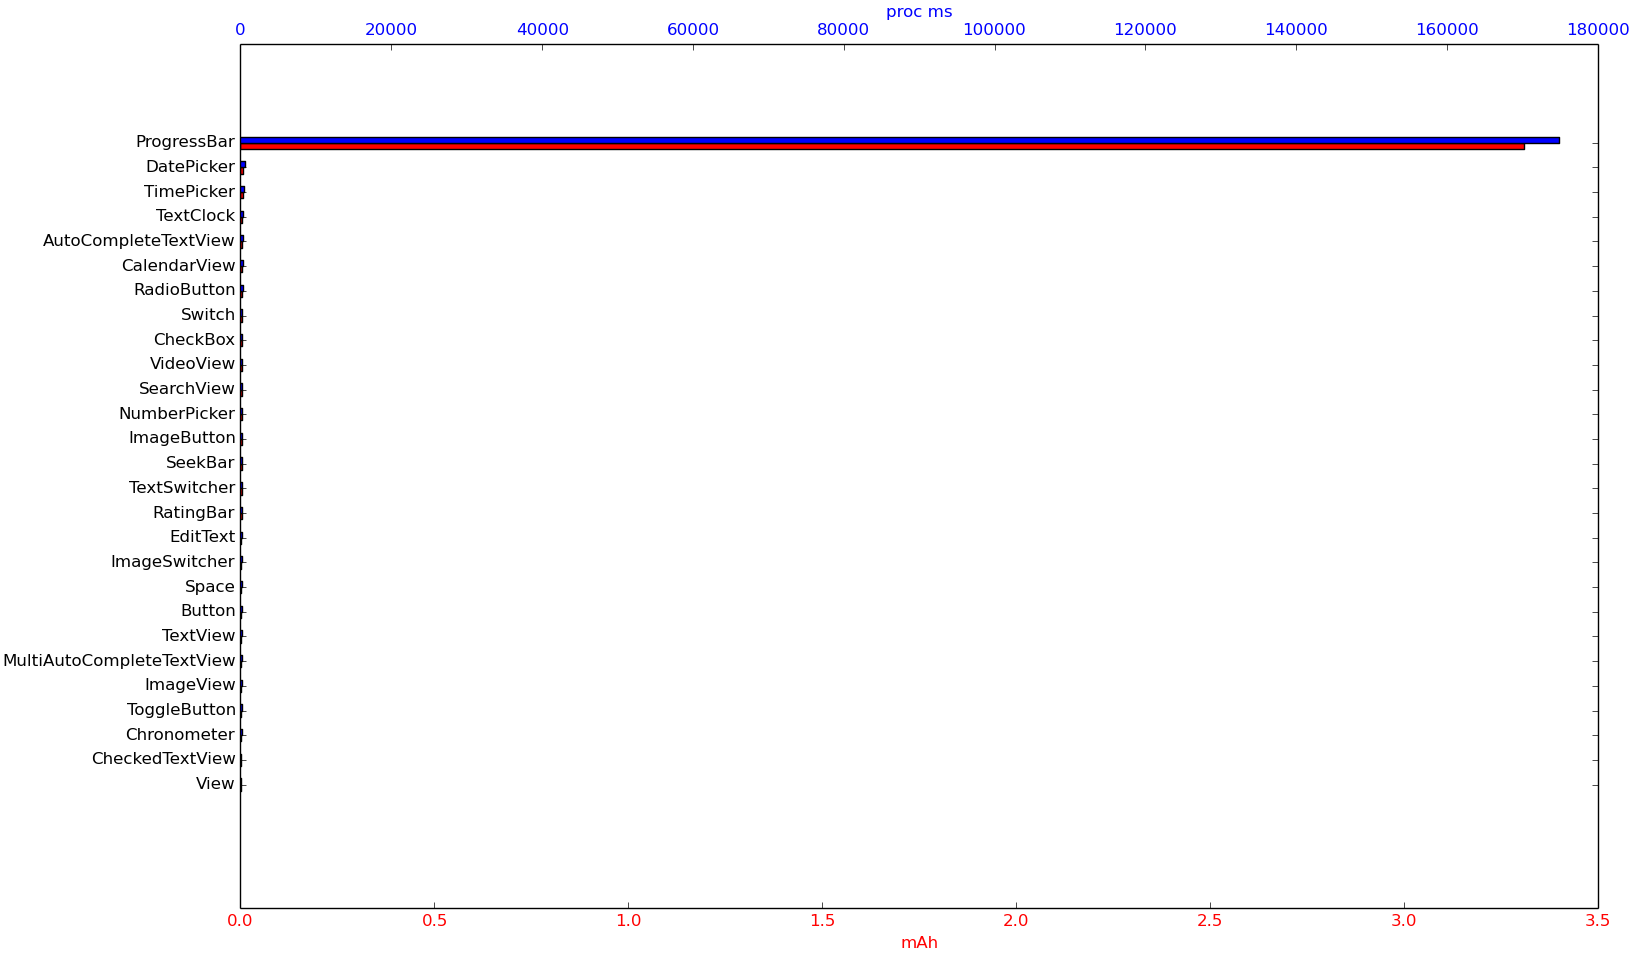
\includegraphics[width=\textwidth]{result}
		\caption{Результаты измерений. Синие столбцы --- процессорное время в мс. Красные столбцы --- количество затраченных mAh.}
		\label{fig:result}
	\end{figure}

	\begin{figure}[!htb]
		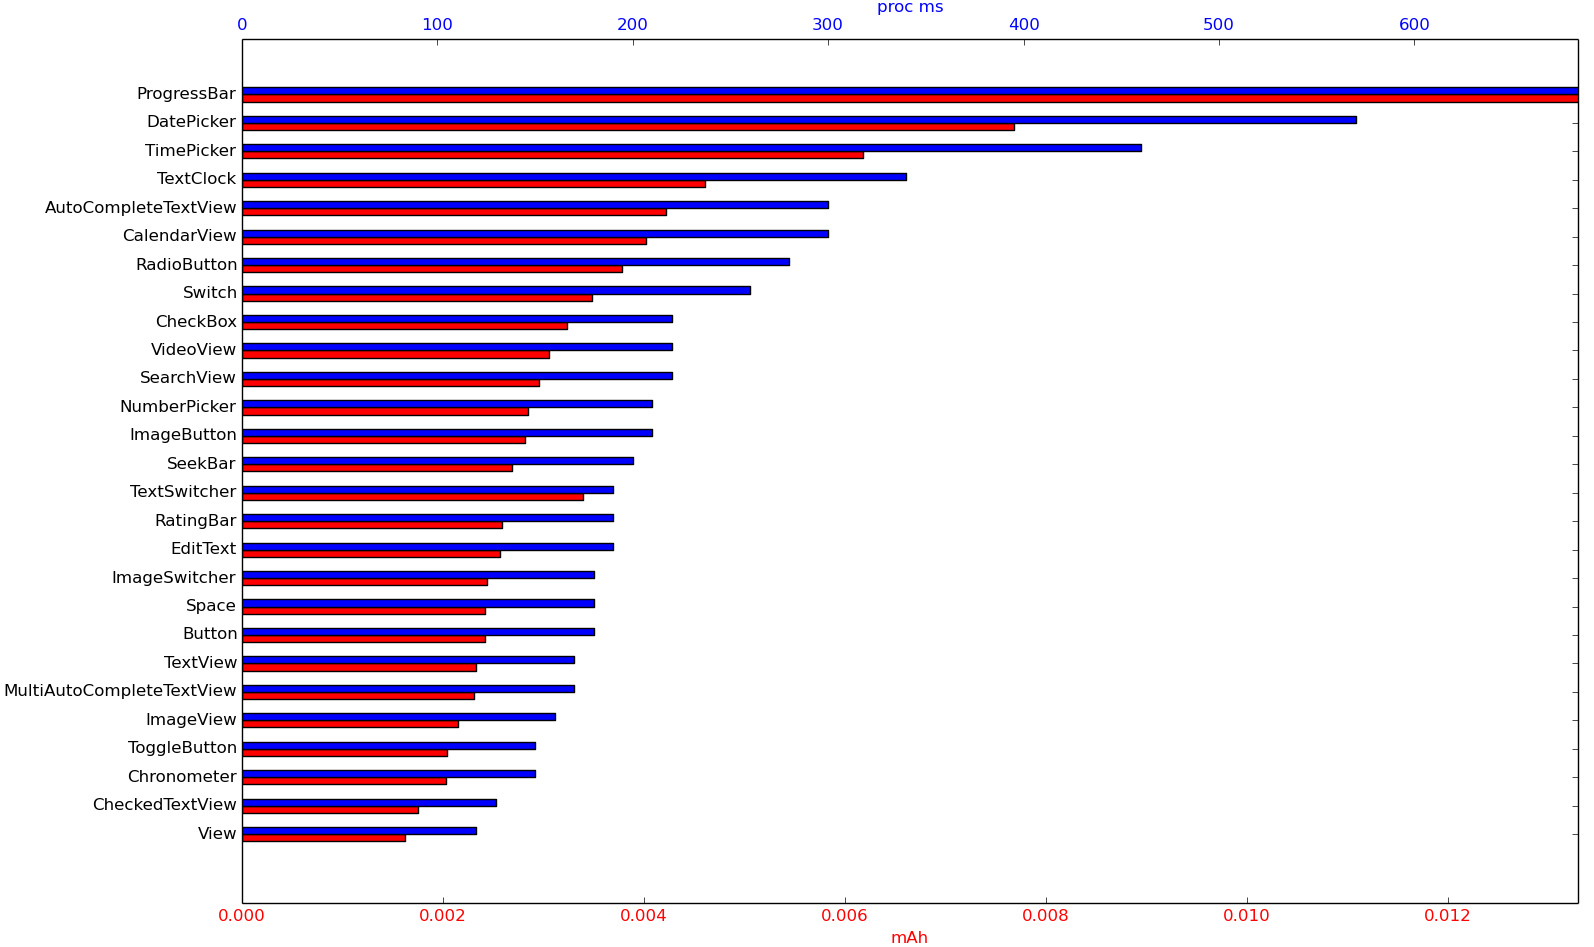
\includegraphics[width=\textwidth]{result_scaled}
		\caption{Результаты измерений. Синие столбцы --- процессорное время в мс. Красные столбцы --- количество затраченных mAh.}
		\label{fig:result_scaled}
	\end{figure}

	Видно, что виджет ProgressBar тратит энергии в десятки раз больше остальных виджетов. Это неудивительно, потому что он проигрывает непрекращающуюся анимацию, которая требует постоянных расчётов и обновления содержимого экрана. Также в движении находится виджет VideoView, который воспроизводит видеофрагмент, но показатели его потребления не выбиваются из ряда остальных.
	
	Из результатов можно сделать и более неожиданные выводы. Например, виджет Space, заявленный как легковесное View, на деле потребляет больше ресурсов устройства, чем оригинальное View. Также MultiAutoCompleteTextView потребляет ощутимо меньше энергии, чем подобные ему AutoCompleteTextView, и даже EditText.
	
	На графике неестественно выглядят показатели потребления TextSwitcher, так как они выбиваются из сортировки. Произошло это из-за выброса показателя потребления в одном из измерений, процессорное время в данном случае отображает более реальные данные.
	
	На основании этих данных удалось составить рекомендацию по оптимизации для 23 виджетов из 27 представленных. Некоторые виджеты не имеют аналогов или уже являются наиболее оптимальными среди аналогичных.
	
	\clearpage
	\section{Подключаемая библиотека}
	
	Теперь можно приступить к написанию библиотеки, которая будет являться конечным результатом работы.
	
	\subsection{Проектирование библиотеки}
	
	Перед написанием кода подключаемой библиотеки, необходимо её спроектировать. Проектирование поможет сделать работу библиотеки более стабильной и готовой к различным изменениям. К тому же, на хорошо спроектированные модули гораздо легче написать тесты при необходимости. 
	
	Задача проектирования заключается в продумывании архитектуры программного продукта, то есть описания того, из каких частей он будет состоять и как они будут между собой связаны. В моём случае библиотека выполняет следующие действия:
	\begin{itemize}
		\item прослушивание событий открытия нового экрана;
		\item прослушивание событий добавления новых элементов на текущий экран;
		\item сравнение заданного элемента интерфейса с его альтернативами на основании базы данных;
		\item вывод результата.
	\end{itemize}

	Изначально кажется, что первые две задачи очень похожи, но на деле это не совсем так, потому что за это отвечают разные механизмы и новый экран может быть открыт несколькими разными способами. Поэтому было решено разделить библиотеку на следующие модули:
	\begin{itemize}
		\item UIManager --- точка входа в программу, которой необходим объект класса Application для установки слушателей открытия нового экрана. Здесь же определяются, какие реализации остальных компонентов будут использованы в работе.
		\item HierarchyAnalyzer --- абстракция с методом analyzeDynamicHierarchy и полями типа Adviser и RecommendationOutputter. Этот класс будет слушать изменения в существующих иерархиях элементов, обращаясь к Adviser, чтобы сравнить элемент с имеющимися в базе данных и к RecommendationOutputter, чтобы вывести полученный результат.
		\item Adviser --- абстракция с методом, который ищет оптимальный элемент, подобный заданному. Может возникнуть необходимость делать это асинхронно, так как поиск будет связан с работой с базой данных, поэтому метод findAlternativeAsync помимо имени класса элемента принимает callback, через который будет возвращён результат.
		\item RecommendationOutputter --- абстракция с методом output, принимающим оригинальный элемент интерфейса и строку с описанием альтернативы.
	\end{itemize}

	Отношения между описанными частями представлены на рис.~\ref{fig:uml_interfaces}.

	\begin{figure}[htb]
		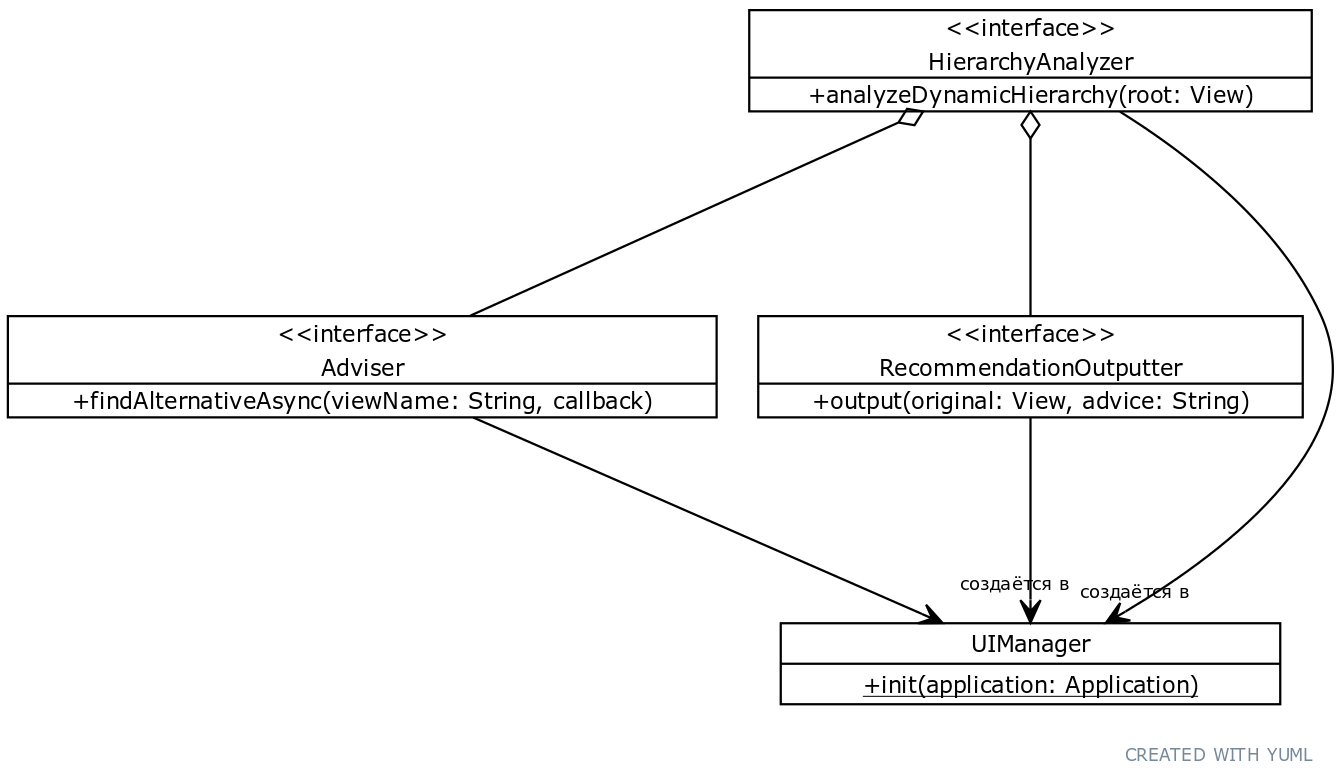
\includegraphics[width=\textwidth]{uml_interfaces}
		\caption{Структурная диаграмма библиотеки}
		\label{fig:uml_interfaces}
	\end{figure}
	
	\subsection{Язык программирования и  инструментальные средства}
	
	Теперь нужно определиться, какими инструментами предстоит пользоваться при написании кода библиотеки. Самое основное --- язык написания программы. Для разработки встраиваемой библиотеки необходимо использовать язык программирования Java и/или Kotlin. Дополнительно могут быть использованы модули, скомпилированные в .so файл, и написанные на любом языке, поддерживающим такую компиляцию. 
	
	Нет необходимости использовать подключение .so файлов в данном проекте, так как здесь не стоит задача обеспечения повышенной производительности и нет потребности в более тонком управлении памятью. Языки Kotlin и Java не имеют разницы в производительности, так как в итоге компилируются в одинаковый байт-код. Различия имеются только в удобстве написания, здесь в большинстве случаев более оптимален Kotlin, позволяющий писать более короткий и более читаемый для человека код. Так как эти языки совместимы, при необходимости можно будет написать фрагмент программы на языке Java, но основным языком разработки был выбран Kotlin.
	
	Так как языки Java и Kotlin совместимы, для написания собственной библиотеки можно использовать другие библиотеки, написанные как на языке Java, так и на языке Kotlin. Сторонние библиотеки могут упростить прослушивание событий, работу с базой данных, реализацию алгоритмов сравнения элементов друг с другом и так далее. Но чтобы не увеличивать размер библиотеки и не добавлять в неё функциональность из сторонней библиотеки, которая не будет использована, было решено пользоваться только средствами Android SDK, а также языков Java и Kotlin.
	
	В библиотеке предстоит отслеживать смену экранов и динамическое изменение иерархий элементов, в Android SDK для этого имеются такие средства как Application.ActivityLifecycleCallbacks, FragmentManager.FragmentLifecycleCallbacks и ViewGroup.OnHierarchyChangeListener. ActivityLifecycleCallbacks используются для отслеживания изменений состояния жизненного цикла Activity. Его удобно использовать, чтобы определять, что создалась новая сущность Activity (для этой сущности будет вызван метод жизненного цикла onCreate). FragmentLifecycleCallbacks может использоваться для отслеживания жизненного цикла Fragment (компонент, который может представлять собой отдельный экран или его часть). OnHierarchyChangeListener в свою очередь позволяет отслеживать динамические изменения иерархии элементов графического интерфейса.
	
	Так как ViewGroup.OnHierarchyChangeListener полностью покрывает все текущие сценарии использования FragmentManager.FragmentLifecycleCallbacks, было решено использовать Application.ActivityLifecycleCallbacks для определения появления новых Activity вместе с ViewGroup.OnHierarchyChangeListener, чтобы находить новые сущности Fragment и вручную добавляемые программистом представления.
	
	\subsection{База данных}
	
	Базу данных решено было спроектировать следующим образом. Существует одна таблица с тремя столбцами. В первом столбце содержится id строки, это поле обязательно. Второй столбец содержит название виджета, для которого в третьем столбце находится название самого близкого по потреблению аналога. Идея состоит в том, чтобы получать самый близкий аналог, потребляющий меньше текущего и выполнять новый поиск для полученного аналога. Таким образом, поиск будет производится до тех пор, пока не будет получен виджет, не имеющий более энергоэффективных аналогов. Результатом станет полный список виджетов, которыми можно заменить текущий виджет, чтобы повысить энергоэффективность приложения.
	
	Иногда нужно дописать какое-либо дополнение к замене, в таких случаях первым словом будет название виджета, а после него дополнение, которое будет добавляться к каждому последующему виджету.
	
	База данных содержит рекомендации по замене следующих виджетов:
	\begin{itemize}
		\item ProgressBar --- Switch
		\item DatePicker --- CalendarView
		\item TimePicker --- AutoCompleteTextView
		\item AutoCompleteTextView – EditText
		\item CalendarView --- EditText
		\item RadioButton --- Switch with custom logic
		\item Switch --- CheckBox
		\item CheckBox --- TextSwitcher
		\item SearchView --- EditText
		\item NumberPicker --- SeekBar
		\item ImageButton --- ImageSwitcher
		\item SeekBar --- EditText
		\item TextSwitcher --- ImageSwitcher
		\item RatingBar --- EditText
		\item EditText --- MultiAutoCompleteTextView
		\item ImageSwitcher --- ToggleButton
		\item Space --- View
		\item Button --- TextView
		\item TextView --- ImageView
		\item MultiAutoCompleteTextView --- ToggleButton
		\item ImageView --- CheckedTextView
		\item ToggleButton --- CheckedTextView
		\item CheckedTextView --- View with background
	\end{itemize}

	Созданная база данных помещена в директорию \textbf{assets} модуля \textbf{hierarchy-checker}, чтобы иметь доступ к бинарному файлу базы из библиотеки.

	\subsection{Разработка}
	
	Перед началом написания кода библиотеки встаёт вопрос организации кода.
	
	\subsubsection{Структура проекта}
	
	Сам проект будет удобно разделить на несколько модулей, чтобы хранить весь код в одном проекте. Модуль \textbf{estimation} содержит весь код, необходимый для проведения измерений. Модуль \textbf{hierarchy-checker} содержит код встраиваемой библиотеки. Модуль \textbf{example} подключает модуль \textbf{hierarchy-checker} и демонстрирует работу библиотеки.
	
	Модуль \textbf{estimation} в корневой директории содержит все используемые скрипты, а также результаты измерений. В директории \textbf{src/androidTest} содержится класс MyTestRunner, а также код автотестов. В директории \textbf{src/main} находятся наследники ViewWrapper, а также класс MainActivity.
	
	\subsubsection{Написание кода библиотеки}
	
	При написании кода было решено начать с описания спроектированной архитектуры в синтаксисе языка программирования Kotlin. UIManager --- singleton-объект, содержащий методы init и getActivityRoot. Первый метод ---  точка входа в приложение, он принимает объект приложения и ничего не возвращает. getActivityRoot принимает на вход объект Activity и возвращает корневое представление иерархии, привязанное к этому Activity. 
	
	Adviser --- интерфейс с методом findAlternativeAsync, который принимает имя класса представления, которое необходимо проанализировать, а также callback, через который будет возвращён результат. RecommendationOutputter тоже интерфейс с методом output, принимающим объект View, для которого сформирована рекомендация, и сама рекомендация в виде строки. 
	
	HierarchyAnalyzer ---  абстрактный класс, у которого имеется конструктор, принимающий реализации Adviser и RecommendationOutputter и сохраняющий их в поля на уровне абстрактного класса. Также он содержит абстрактный метод analyzeDynamicHierarchy, который принимает корень иерархии элементов, которую необходимо проанализировать.
	
	Реализация HierarchyAnalyzer содержит объект OnHierarchyChangeListener, который она передаёт всем объектам ViewGroup, встречающимся в иерархии. Для прохода иерархии используется итерация по всем дочерним элементам корневого элемента и рекурсивного вызова analyzeDynamicHierarchy в случае, если дочерний элемент также может содержать дочерние элементы. Реализация OnHierarchyChangeListener вызывает метод analyzeDynamicHierarchy для каждого динамически добавленного элемента.
	
	В качестве реализации интерфейса RecommendationOutputter используется LogOutputter, выводящий информацию в логи устройства. При вызове метода output реализация проходит по всем родительским элементам, чтобы составить полный адрес текущего элемента в иерархии. Для смены порядка родительских элементов (идём снизу вверх по иерархии, выводим её сверху вниз) используется стек. После этого формируется сообщение, содержащее класс объекта, его расположение в иерархии и совет по оптимизации. Сообщение выводится в логи устройства.
	
	Класс DatabaseAdviser реализует интерфейс Adviser и содержит в поле класса объект AdviceHelper, который абстрагирует взаимодействие с базой данных, а также ThreadPoolExecutor, который сохраняет несколько потоков исполнения, которые могут быть многоразово использованы или завершены, если дополнительных задач не поступает в течение 30 секунд. Предполагается, что его использование сократит издержки на создание новых потоков за счёт переиспользования уже существующих. 
	
	При вызове метода findAlternativeAsync на потоке, который предоставляет объект ThreadPoolExecutor, вызывается метод getAdvice у AdviceHelper, который возвращает более эффективный аналог. Но чтобы сформировать наиболее полный список аналогов, метод getAdvice вызывается ещё раз для результата предыдущего вызова. Так происходит до тех пор, пока программа не достигнет самого оптимального виджета. Все виджеты будут описаны в результате, который уже на главном потоке передаётся в переданный методу callback. В иерархии реального приложения некоторые названия виджетов могут отличаться от того, что есть в базе данных. Например, вместо TextView можно встретить AppCompatTextView. Такая замена совершается операционной системой и предусматривается алгоритмами поиска в базе данных.
	
	Класс AdviceHelper наследует SQLiteOpenHelper и инкапсулирует всю работу с базой данных. Одна из главных задач, которую он решает, это использование заранее готовой базы данных. Изначально база данных находится в специальном месте для бинарных файлов, но использовать её из этой директории нельзя, так как SQLiteOpenHelper работает только с базами, созданными самим приложением, и находящимися в отдельной директории. Чтобы решить эту задачу, при инстанциировании AdviceHelper проверяет, существует ли база данных, созданная приложением. Если такой нет, значит запуск библиотеки с этим приложением происходит впервые. В этом случае файл базы копируется из изначальной директории в директорию с базами данных приложения. Если база уже существует, открывается соединение с ней для проверки её версии. Если версия совпадает с ожидаемой, база закрывается, если нет, база, возможно, устарела. В случае устаревшей базы данных, она удаляется и заново копируется из директории с оригинальным файлом, который мог измениться.
	
	В методе init класса UIManager создаются конкретные реализации Adviser и RecommendationOutputter, они передаются в конструктор ConcreteHierarchyAnalyzer. Затем на объекте приложения вызывается registerActivityLifecycleCallbacks, а в реализации Application.ActivityLifecycleCallbacks при приобретении какой-либо Activity состояния Started, с помощью метода getActivityRoot находится корень его иерархии и передаётся в метод analyzeDynamicHierarchy созданного ранее HierarchyAnalyzer.
	
	Итоговая библиотека имеет структуру, представленную на рис~\ref{fig:uml}.
	
	\begin{figure}[htb]
		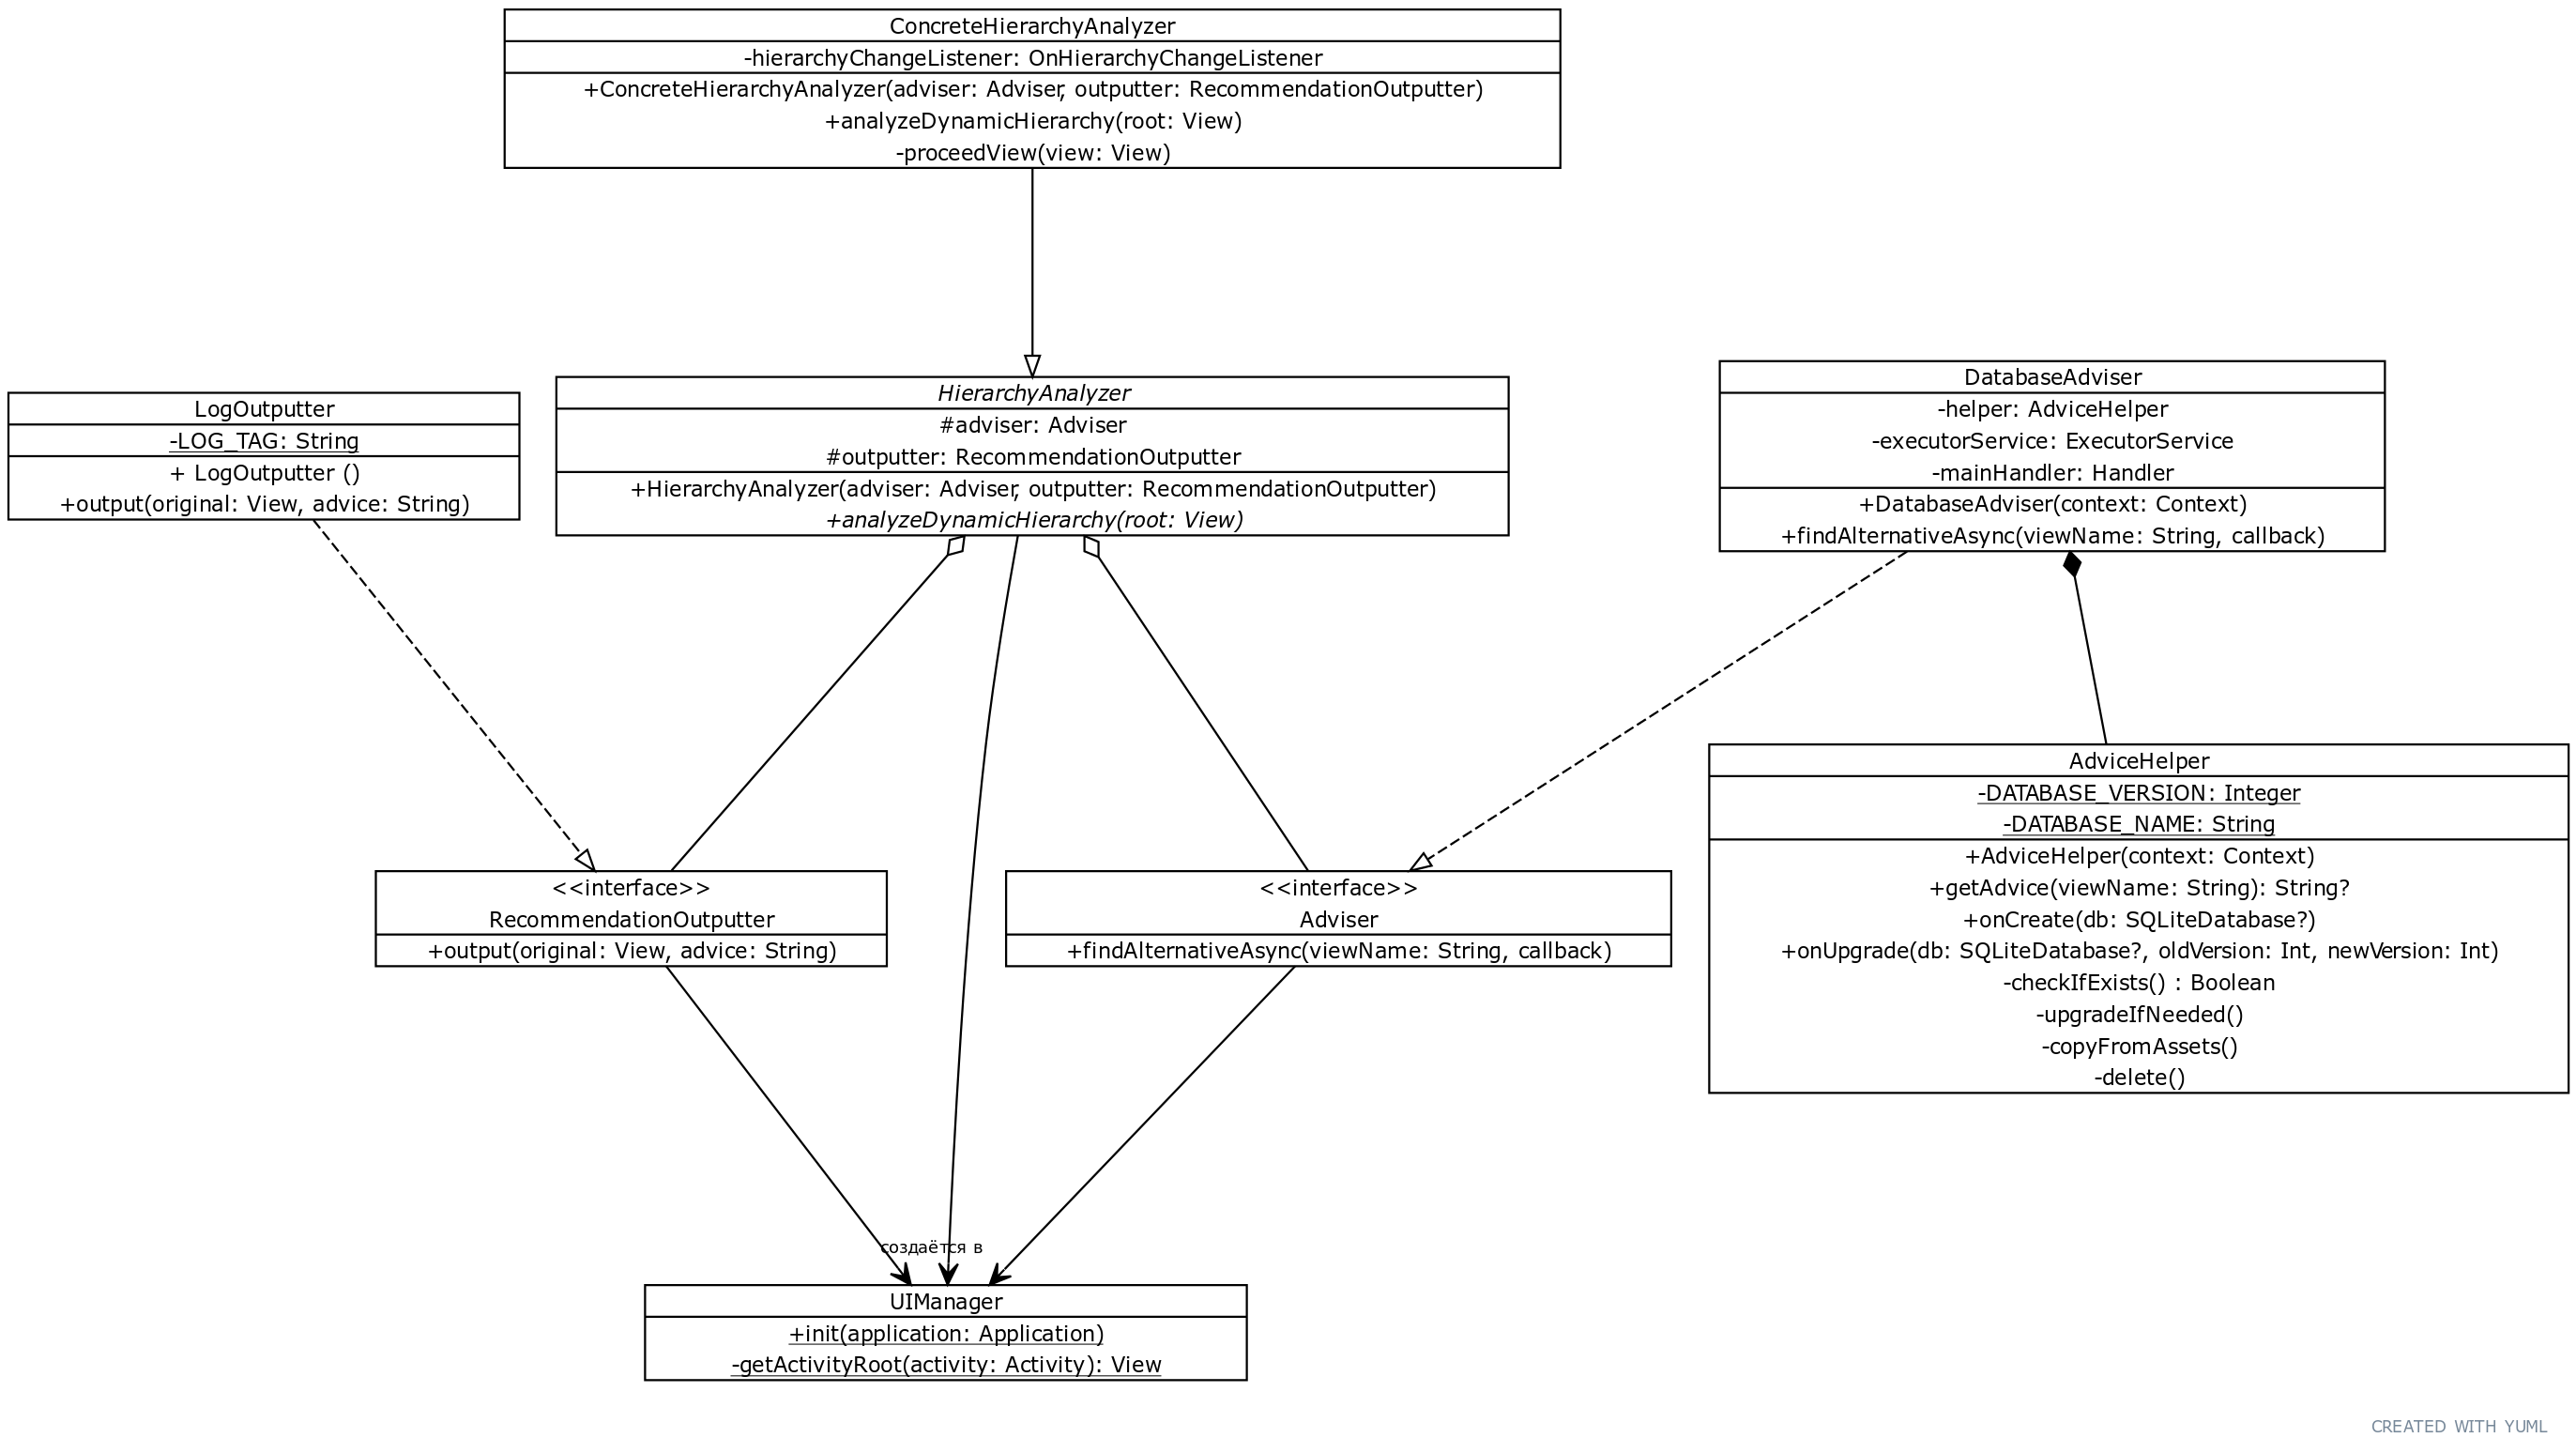
\includegraphics[width=\textwidth]{uml}
		\caption{Диаграмма классов библиотеки}
		\label{fig:uml}
	\end{figure}
	
	\newpage
	\section{Итоги работы}
	
	Весь исходный код проекта, а также необработанные результаты всех проведённых измерений были опубликованы на GitHub~\parencite{GitHub}.
	
	Для демонстрации работы библиотеки в проект был добавлен модуль \textbf{example}. Модуль содержит приложение, способное динамически добавлять на экран объект класса \textbf{android.app.Fragment} с наполнением, объект класса \textbf{androidx.fragment.app.Fragment} с наполнением, объекты класса \textbf{TextView}, а также открывать новое Activity~\ris{\ref{fig:example}}. К проекту подключена библиотека из модуля \textbf{hierarchy-checker} и в методе onCreate наследника класса Application у объекта UIManager был вызван метод init, в который был передан контекст приложения.
	
	\begin{figure}[htb]
		\centering
		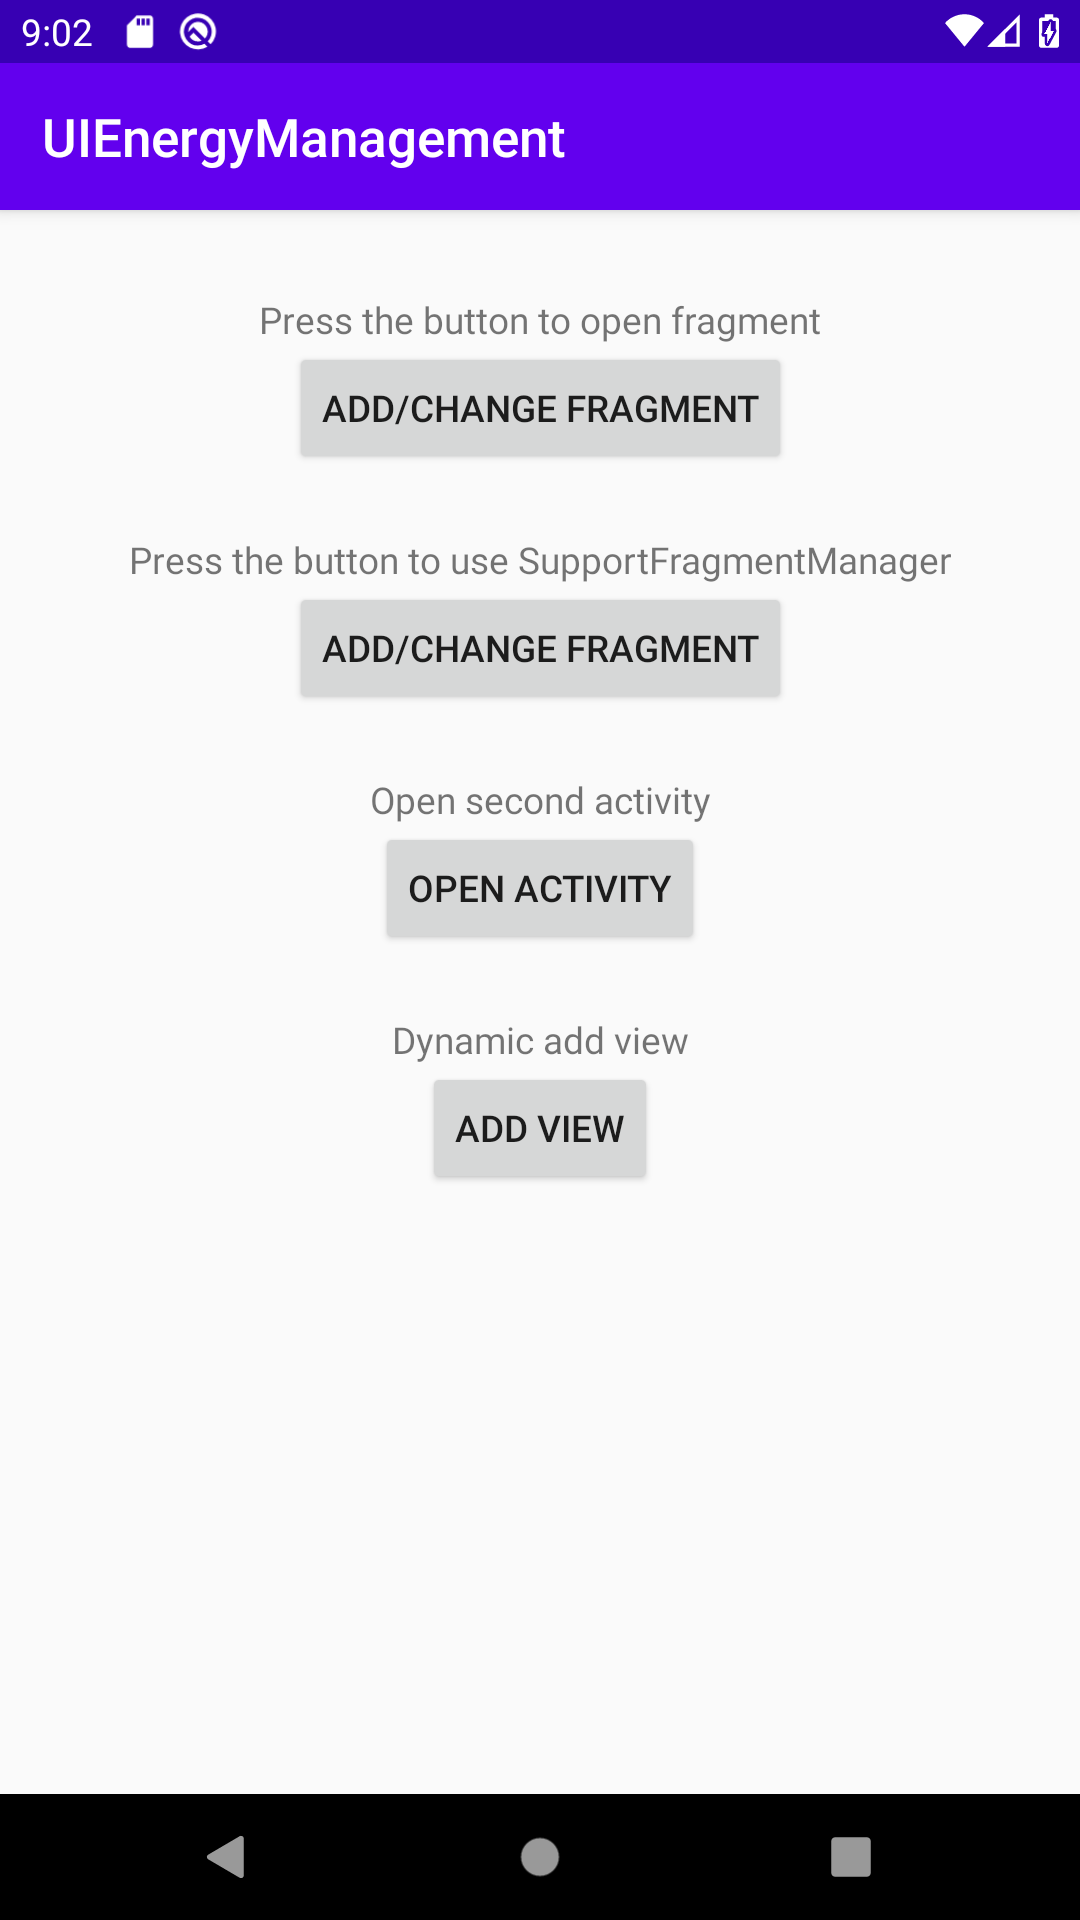
\includegraphics[width=0.45\textwidth]{example}
		\caption{Интерфейс приложения из модуля example}
		\label{fig:example}
	\end{figure}
	
	Так как главный экран приложения уже содержит кнопки и текстовые поля, сразу после открытия приложения в логах устройства появляются советы по оптимизации открывшегося экрана~\ris{\ref{fig:example_log}}.
	
	\begin{figure}[htb]
		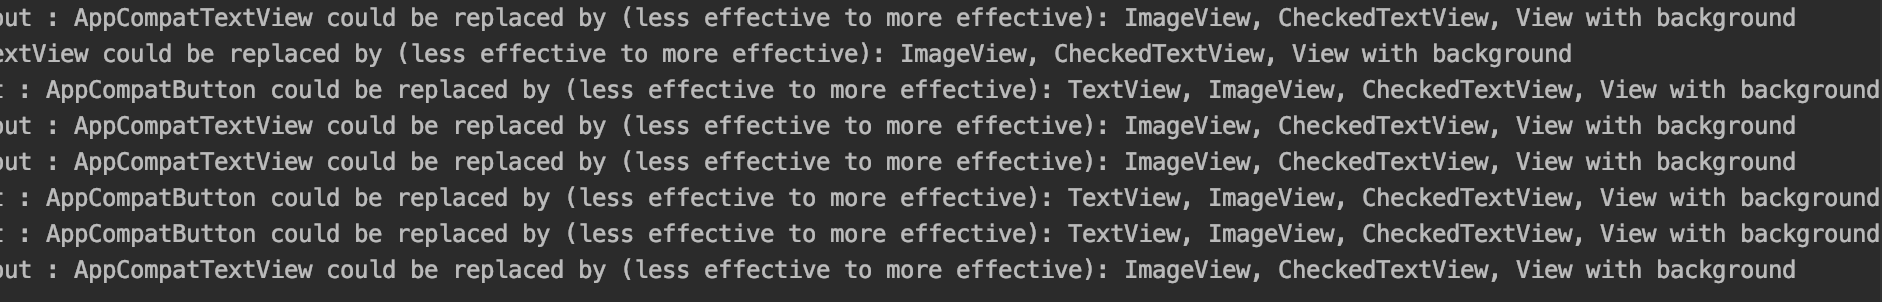
\includegraphics[width=\textwidth]{example_log}
		\caption{Логи устройства после открытия приложения из модуля example}
		\label{fig:example_log}
	\end{figure}

	При нажатии кнопок на экран добавляются новые виджеты или открывается новый экран. При этом библиотека находит новые виджеты в иерархии и сразу после их отображения выводит в логи устройства советы по оптимизации, если их удалось найти в базе данных.
	
	\newpage
	\centertitletoc{Заключение}
	
	Для разработки системы контроля и управления энергопотреблением элементов графического интерфейса на устройствах под управлением операционной системы Android были проведены измерения 27 виджетов в пакете android.widget в Android 10 SDK Platform. Результаты измерений показали соотношения энергопотребления между всеми измеренными элементами.
	
	На основании результатов измерений была составлена база данных, которая используется встраиваемой библиотекой для формирования советов по уменьшению энергопотребления приложения. Это позволит разработчикам приложений выявлять неэффективные с точки зрения энергопотребления виджеты приложения получать советы по их оптимизации.
	
	Существенными ограничениями данной работы являются следующие факторы:
	\begin{itemize}
		\item Отсутствие доступа к стороннему оборудованию для измерения энергопотребления;
		\item Отсутствие доступа к устройству без сторонних приложений и без служб Google Play Services;
		\item Наличие лишь одного устройства для тестирования.
	\end{itemize}

	Изначально для измерения энергопотребления устройства планировалось использовать специализированное оборудования Monsoon Power Monitor. Использование данного оборудования позволило бы более точно измерить энергопотребление устройства, причём не за всё время тестирования виджета, а за более малые промежутки. Инструмент Battery Historian также имеет возможность обработки результатов работы Monsoon Power Monitor. В дальнейших исследованиях можно повторить измерения с использованием более точного стороннего оборудования.
	
	Отсутствие сторонних приложений на тестируемом устройстве могло бы снизить искажения проводимых измерений, так как приложения могут совершать фоновую работу. Часть затраченных ресурсов операционная система разделяет на все запущенные в данный момент приложения и результаты измерений могут быть искажены. Службы Google Play Services --- одна из главных составляющих фонового потребления ресурсов устройства, поэтому тестирование оптимальнее проводить на устройстве без данных служб. Их отличие от приложений состоит в том, что службы предустановлены в операционную систему и не могут быть удалены или отключены обычным пользователем.
	
	Некоторые искажения могут быть связаны с моделью устройства, используемого для тестирования, или с версией операционной системы, установленной на нём. Для получения более объективных показателей требуется проведение тестирования на нескольких устройствах и обобщение результатов.

	В дальнейших исследованиях может быть увеличено количество проводимых измерений, виджеты во время тестирования могут перерисовываться вызовом метода invalidate, а также может быть сымитировано пользовательское взаимодействие с устройством.
	
	\newpage
	\centertitletoc{Глоссарий}
	
	База данных --- организованная структура, которая используется для хранения, обработки и изменения взаимосвязанной информации.
	
	Библиотека --- набор ресурсов, используемых для разработки программного обеспечения.
	
	Виджет --- элемент графического интерфейса, используемый на экране приложения.
	
	Фреймворк автоматического тестирования --- программное обеспечение, позволяющее создавать тесты для автоматизированного тестирования приложения. Частные случаи: appium, espresso, kakao, kaspresso.
	
	Activity --- компонент приложения, имеющий графический интерфейс, и позволяющий пользователю с ним взаимодействовать.
	
	Android --- мобильная операционная система с открытым исходным кодом.
	
	Android Debug Bridge --- инструмент командной строки, позволяющий взаимодействовать с устройством.
	
	Android Profiler --- инструмент, предоставляющий данные о потребляемых приложением ресурсах устройства в реальном времени.
	
	Battery Historian --- инструмент анализа и визуализации расхода батареи устройства на основании отчётов операционной системы.
	
	BroadcastReceiver --- компонент приложения, позволяющий принимать и обрабатывать системные события.
	
	Uid --- пользовательский идентификатор в Unix-подобных операционных системах, он уникален для каждого приложения и по нему можно отслеживать потребление.

	\newpage
	\centertitletoc{Перечень сокращений, условных обозначений, символов и терминов}
	
	Автотест --- тест для автоматизированного тестирования приложения.
	
	ОС --- операционная система.
	
	adb --- Android Debug Bridge.
	
	API --- application program interface.
	
	mAh --- миллиампер-час.
	
	zsh --- Z shell.
	
	\newpage
	\centertitletoc{Список использованных источников}
	
	\printbibliography[heading=none]
	
	\newpage
	\begin{flushright}
		\phantomsection
		\addcontentsline{toc}{section}{Список сущностей пакета android.widget в Android 10 SDK Platform}
		\label{appendix}
		Приложение\par
		Список сущностей пакета android.widget в Android 10 SDK Platform
	\end{flushright}

	\begin{itemize}
        \item AbsListView
        \item AbsoluteLayout
        \item AbsSeekBar
        \item AbsSpinner
        \item ActionMenuView
        \item Adapter
        \item AdapterView
        \item AdapterViewAnimator
        \item AdapterViewFlipper
        \item Advanceable
        \item AlphabetIndexer
        \item AnalogClock
        \item ArrayAdapter
        \item AutoCompleteTextView
        \item BaseAdapter
        \item BaseExpandableListAdapter
        \item Button
        \item CalendarView
        \item Checkable
        \item CheckBox
        \item CheckedTextView
        \item Chronometer
        \item CompoundButton
        \item CursorAdapter
        \item CursorTreeAdapter
        \item DatePicker
        \item DialerFilter
        \item DigitalClock
        \item EdgeEffect
        \item EditText
        \item ExpandableListAdapter
        \item ExpandableListView
        \item Filter
        \item Filterable
        \item FilterQueryProvider
        \item FrameLayout
        \item Gallery
        \item GridLayout
        \item GridView
        \item HeaderViewListAdapter
        \item HeterogeneousExpandableList
        \item HorizontalScrollView
        \item ImageButton
        \item ImageSwitcher
        \item ImageView
        \item LinearLayout
        \item ListAdapter
        \item ListPopupWindow
        \item ListView
        \item Magnifier
        \item MediaController
        \item MultiAutoCompleteTextView
        \item NumberPicker
        \item OverScroller
        \item PopupMenu
        \item PopupWindow
        \item ProgressBar
        \item QuickContactBadge
        \item RadioButton
        \item RadioGroup
        \item RatingBar
        \item RelativeLayout
        \item RemoteViews
        \item RemoteViewsService
        \item ResourceCursorAdapter
        \item ResourceCursorTreeAdapter
        \item Scroller
        \item ScrollView
        \item SearchView
        \item SectionIndexer
        \item SeekBar
        \item ShareActionProvider
        \item SimpleAdapter
        \item SimpleCursorAdapter
        \item SimpleCursorTreeAdapter
        \item SimpleExpandableListAdapter
        \item SlidingDrawer
        \item Space
        \item Spinner
        \item SpinnerAdapter
        \item StackView
        \item Switch
        \item TabHost
        \item TableLayout
        \item TableRow
        \item TabWidget
        \item TextClock
        \item TextSwitcher
        \item TextView
        \item ThemedSpinnerAdapter
        \item TimePicker
        \item Toast
        \item ToggleButton
        \item Toolbar
        \item TwoLineListItem
        \item VideoView
        \item ViewAnimator
        \item ViewFlipper
        \item ViewSwitcher
        \item WrapperListAdapter
        \item ZoomButton
        \item ZoomButtonsController
        \item ZoomControls
	\end{itemize}
\end{document}
